\documentclass[a4paper,11pt,twoside,openright]{book}
\usepackage[T1]{fontenc}
\usepackage[title,toc,page]{appendix}
\usepackage[cp1250]{inputenc}  
\usepackage{amsmath} 
\usepackage{amssymb} 
\usepackage{epsfig} 
\usepackage[inner=3cm,outer=2cm]{geometry} 
\usepackage{cite}
\usepackage{graphicx}
\usepackage{caption}
\usepackage{subcaption}
\usepackage{sidecap}
\usepackage{float}
\usepackage{url}
\usepackage{multirow}
\usepackage{array}
\usepackage{mathrsfs}
\usepackage{lscape}
\usepackage{xcolor}
\usepackage{colortbl}
\usepackage{array}
%\usepackage{showframe}
%\usepackage{setspace}
%\setstretch{1.1}

\newcommand{\cvut}{Czech Technical University in Prague}
\newcommand{\fjfi}{Faculty of Nuclear Sciences and Physical Engineering}
\newcommand{\km}{Department of Physics}
\newcommand{\obor}{Mathematical Engineering}
\newcommand{\oborcz}{Matematick\'{e} In\v{z}en\'{y}rstv\'{i}}
\newcommand{\zamereni}{Mathematical Physics}

\newcommand{\nazevcz}{Jety s vysokou p\v{r}\'{i}\v{c}nou hybnost\'{i} v RunII experimentu ATLAS}        
\newcommand{\nazeven}{High $\pt$ jets in RunII of the ATLAS Experiment}    
\newcommand{\autor}{Jan Lochman}          
\newcommand{\rok}{May 2015}         
\newcommand{\vedouci}{Ing. Zden\v{e}k Hub\'{a}\v{c}ek, Ph.D.}        
\newcommand{\pracovisteVed}{CERN}	

\newcommand{\klicova}{Klicova slova}   
\newcommand{\keyword}{Keywords}

\newcommand{\abstrCZ}{Abstrakt CZ} 
\newcommand{\abstrEN}{
This thesis deals with the meassurement of the inclusive jet double differential
cross section in $\pt$ and rapidity using \textsc{Pythia8} generated events of
$pp$ colisions at $\sqrt{s} = 13 \, \text{TeV}$ with the ATLAS detector response
reconstructed by \textsc{Geant4} detector simulation. Differential cross
section obtained from the detector level is unfolded on the particle level
and compared with the parton level cross section prediction of the NLO pQCD.
Both \textsc{Pythia8} and NLO pQCD have used CT10 PDFs and ATLAS underlying
event tune AU2.  
}

\newcommand{\MyQuote}[2]{
  \begin{center}
    \textit{\quotation{#1}}
  \end{center}
  \begin{flushright}
    #2
  \end{flushright}
  \vspace{10mm}
}

\newcolumntype{L}[1]{>{\raggedright\let\newline\\\arraybackslash\hspace{0pt}}m{#1}}
\newcolumntype{C}[1]{>{\centering\let\newline\\\arraybackslash\hspace{0pt}}m{#1}}
\newcolumntype{R}[1]{>{\raggedleft\let\newline\\\arraybackslash\hspace{0pt}}m{#1}}

\newcommand{\TeV}{\,\text{TeV}}
\newcommand{\GeV}{\,\text{GeV}}
\newcommand{\MeV}{\,\text{MeV}}
\newcommand{\pt}{p_{T}}
\newcommand{\Euler}{\mathrm{e}}
\newcommand{\rts}{\sqrt{s}}



\begin{document}

%================================================================================
% Title page
%================================================================================
\thispagestyle{empty}

\begin{center}
    {\Large \textsc{\cvut}\\[1.5ex] \textsc{\fjfi}}\\[1.5ex]{\large \textsc \km}
    \vspace{10mm}

    \begin{tabular}{c}
    {Programme: \obor}\\
    {Branch of Study: \zamereni}
    \end{tabular}

    \vspace{10mm} \epsfysize=25mm \epsffile{cvut} \epsfysize=25mm \epsffile{fjfi} \vspace{15mm}
    %\vspace{50mm}

   {\huge \bf \nazeven}

   \vspace{15mm}
   {\Large MASTER'S DEGREE PROJECT}

   \vfill
   {\large
    \begin{tabular}{ll}
    Author: & \autor\\
    Supervisor: & \vedouci\\
    Submitted in: & \rok
    \end{tabular}
   }
\end{center}


%================================================================================
% Empty page
%================================================================================
\newpage  
\thispagestyle{empty} 
~


%================================================================================
% Official assignment
%================================================================================
\newpage  
\thispagestyle{empty} 
Zadani prace


%================================================================================
% Empty page
%================================================================================
\newpage  
\thispagestyle{empty} 
~


%================================================================================
% Statement
%================================================================================
\newpage 
\thispagestyle{empty}  
~
\vfill 
{\bf Statement} 

\vspace{0.5cm} 
Prohlasuji\ldots

\vspace{5mm}V Praze dne ....................\hfill 
............................................       
\begin{flushright}
  \autor 
\end{flushright}

\newpage 
\thispagestyle{empty}  
~
   
%================================================================================
% Acknowledgment
%================================================================================
\newpage 
\thispagestyle{empty}  
~
\vfill 
{\bf Acknowledgment} 

\vspace{0.5cm} 
Dekuji\ldots

\begin{flushright}
  \autor 
\end{flushright}

\newpage 
\thispagestyle{empty}  
~

%================================================================================
% Abstract and others
%================================================================================
\newpage   
\thispagestyle{empty} 

\newbox\odstavecbox
\newlength\vyskaodstavce
\newcommand\odstavec[2]{%
    \setbox\odstavecbox=\hbox{%
         \parbox[t]{#1}{#2\vrule width 0pt depth 4pt}}%
    \global\vyskaodstavce=\dp\odstavecbox
    \box\odstavecbox}
\newcommand{\delka}{120mm} 

\begin{tabular}{ll}
  {\em N\'{a}zev pr\'{a}ce:} & ~ \\
  \multicolumn{2}{l}{\odstavec{\textwidth}{\bf \nazevcz}} \\[0.2em]
  {\em Autor:}                 & \autor \\[0.2em]
  {\em Obor:}                  & \oborcz \\[0.2em]
  {\em Druh pr\'{a}ce:}        & Diplomov\'{a} pr\'{a}ce \\[0.2em]
  {\em Vedouc\'{i} pr\'{a}ce:} & \odstavec{\delka}{\vedouci \\ \pracovisteVed} \\[0.2em]
  \multicolumn{2}{l}{\odstavec{\textwidth}{{\em Abstrakt:} ~ \abstrCZ  }} \\[0.2em]
  {\em Kl\'{i}\v{c}ov\'{a} slova:} & \odstavec{\delka}{\klicova} \\[2em]

  {\em Title:} & ~\\
  \multicolumn{2}{l}{\odstavec{\textwidth}{\bf \nazeven}}\\[0.2em]
  {\em Author:} & \autor \\[0.2em]
  \multicolumn{2}{l}{\odstavec{\textwidth}{{\em Abstract:} ~ \abstrEN  }} \\[0.2em]
  {\em Key words:} & \odstavec{\delka}{\keyword}
\end{tabular}


\newpage 
\thispagestyle{empty}  
~

%================================================================================
% Content
%================================================================================
\clearpage
\pagenumbering{roman}
\setcounter{page}{1}
\tableofcontents 

%================================================================================
% Tabulky
%================================================================================
\clearpage
\addcontentsline{toc}{chapter}{\listtablename}
\listoftables

%================================================================================
% Obrazky
%================================================================================
\clearpage
\addcontentsline{toc}{chapter}{\listfigurename}
\listoffigures

\cleardoublepage

%================================================================================
% Chapters
%================================================================================
\clearpage
\pagenumbering{arabic}
\setcounter{page}{1}

\chapter*{Introduction}
\addcontentsline{toc}{chapter}{Introduction}

Search for the superior equation which would be able to explain all about the
physical universe we do observe, sometimes called the Theory of Everything, led
physicists to the concept of elementary particles some of which define the
building blocks of our observable universe whereas the remaining govern the way how
they interact. 

From the beginning of the 20$^{th}$ century, the term of elementary particles
was redefined with new generation of physicists as is illustrated in Figure
\ref{fig:HistoryOfElPartPhysics}. The latest reform was caused by quarks and the
invention of Quantum Chromodynamics describing its strong interaction which is
next to the electromagnetic and weak interactions encapsulated by the present
theory of elementary particles called the Standard Model. 

\begin{figure}[t]
  \centering
  \includegraphics[width=\textwidth]{Introduction/HistoryOfElementaryParticlePhysics.png}
  \caption{History of elementary particle physics. Figure From
    \cite{LatticeQCDForPedestrians}.}
  \label{fig:HistoryOfElPartPhysics}
\end{figure}

Although Standard Model contains mechanism for assigning elementary particles
masses, gravity was not included in Standard Model up to date because the
present attempts of quantization gravity and description gravity as the
interaction mediated by the quanta of gravity, known as gravitons, led to the
unrenormalizable theories. There are others by the Standard Model unresolved
questions including the nature of the dark part of our universe and the origin
of the matter-antimatter asymmetry. 


%Humans have build large particle accelerators to verify, if the Standard Model
%is the correct theory of particle physics. Next to these experiments, the huge
%telescopes on the Earth as well as in the orbit are looking to the distant
%galaxies.  Although Standard Model have with the help of supercomputers
%succeeded in explanation of the structure and origin of recently observed
%objects (pulsars, neutron stars) and the description of Supernovas, the new
%yet unexplained phenomenons emerged including dark matter and dark energy.

%Standard Model in its present form is not able to explain what these dark
%substances of our universe are. Fortunately there are some theories or better -
%some extensions of Standard Model - which could have answer. These include the
%Supersymmetry or the theories of Extra Dimensions. 

Although it is sure, the Standard Model is not the ultimate Theory of
Everything, it successfully stands against present results from particle
accelerators. 
Last discoveries in particle physics occured on $\sim 100\GeV$ energy
scale with top quark discovery (?citace?) with mass $173.34 \pm 0.98 \GeV$ in 1995
at Tevatron and Higgs boson discovery (?citace?) with mass $125.09 \pm 0.32
\GeV$ in 2012 at CERN and both were successfully predicted by the Standard
Model. If there is new physics beyond the Standard Model on $\sim \TeV$ scale,
the LHC Run II could be the first to discover it \cite{PhysicsAtRun2LHC}. 

This thesis deals with the measurement of double differential inclusive jets 
cross section in $\pt$ and rapidity.  Inclusive jets are the dominant objects
observed on hadron colliders dominating any other observable physics process in
orders of magnitude and could thus be the one of the first indicators of new
physics. 

First Chapter deals with the Quantum Chromodynamics and follows the historical
development including experiments which led to the removing proton from the list
of elementary particles and replacing it by the quarks. QCD will be formulated
as the quantum field theory and the phenomenon known as the running coupling
constant will be discussed. This will lead to the division of the QCD into
perturbative and non-perturbative regions.

In the second Chapter, the Large Hadron Collider will be encountered with
detailed description of its largest ATLAS detector. The basic features of QCD
introduced in the previous chapter will be used to define jets - objects we do
dominantly observe on hadron colliders. The jet reconstruction on ATLAS detector
including description of jet calibration and unfolding of observed spectra will
be presented in this chapter as well.

Third chapter describes the steps of analysis.


\chapter{QCD}
\label{ch:qcd}

\MyQuote{Is the purpose of theoretical physics to be no more than a cataloging of all the
things that can happen when particles interact with each other and separate? Or
is it to be an understanding at a deeper level in which there are things that
are not directly observable (as the underlying quantized fields are) but in
terms of which we shall have a more fundamental understanding?}
{Julian Schwinger}

The theoretical framework of particle physics is called the Standard Model (SM). The
SM describes the way how the fundamental components of matter interact with each
other through strong, weak and electromagnetic interactions. Mathematically the
SM is gauge quantum field theory with local internal symmetries of the direct
product group $SU(3) \times SU(2) \times U(1)$. Gauge bosons are assigned to
generators of this symmetry - there are 8 massless gluons from $SU(3)$ and 3
massive $W^\pm, Z$ bosons with 1 massless boson $\gamma$ from electroweak $SU(2)
\times U(1)$ sector. Higgs mechanism has to be introduced in the electroweak sector
to assign $W^\pm, Z$ bosons mass and as consequence the new particle - Higgs
boson - emerges in the SM theory. All bosons have integer spin. 

In addition to the bosons the SM introduces spin$1/2$ fermions which are
divided into three quark and three lepton families. Fermions are assumed to be
point-like because there is no evidence for their internal structure to date.
All fermions interact weakly, if they have electrical charge, they interact
electromagnetically as well. Quarks are the only fundamental fermions which do
interact strongly. System of fundamental particles of the SM is shown in Figure
\ref{fig:SMparticles}. 

\begin{figure}[!ht]
  \centering
  \includegraphics[width=\textwidth]{Chapter1/SM.png} 
  \caption{The system of fundamental particles of the SM. Figure from
    \cite{wiki:SMParticlesSource}}
  \label{fig:SMparticles}
\end{figure}

Quarks bind together to form hadrons and there are hundreds
\cite{PDG:ReviewOfParticlePhysics} of known hadrons up to date. Hadrons are
divided into baryons (3 quarks) and mesons (quark and anti-quark pairs). Theory
describing the interaction between quarks is called Quantum Chromodynamics (QCD)
which key features will be discussed in this chapter. The reasoning for quark
existence and for the description their strong interaction as $SU(3)$ gauge
theory will be presented. Running coupling constant will be discussed to split
QCD into perturbative and non-perturbative regions - two regions, where QCD has
to use different mathematical approach for the description of strong
interaction. Most of ideas presented here is overtaken from the following
textbook \cite{QCDTextbook}. Electroweak sector of the SM is described in
\cite{horejsi2002fundamentals}. For more concise information about the SM the
following textbooks can serve
\cite{griffiths2008introduction,cottingham2007introduction}.

\section{Theoretical Ansatz}
\label{Sec:TheoreticalAnsatz}

In 1950s, there have already been discovered tens of new hadrons thanks to new
particle accelerators and a lot of effort was exerted to categorize them. To each
particle there was assigned a series of quantum numbers
including isospin $T$ with its third component $T_3$, hypercharge $Y$,
electrical charge $Q$, strangeness $S$, baryon number $B$ and others. Soon it
was recognized, that there are some symmetries between these quantum numbers,
like famous Gell-Mann--Nishijima relation
\cite{GellMannNishijima1,GellMannNishijima2}

\begin{equation}
  Q = T_3 + 1/2 Y \quad , \quad Y = B + S + \dots,
  \label{ex:GellMannNishijima}
\end{equation}
where dots denote charm, bottomness and topness and were introduced after work
of Gell-Mann and Nishijima. Some of the baryons known by then are shown in table
\ref{tab:SelectedHadrons}. In 1960s, the known hadrons were successfully
categorized with the so called Eightfold Way, which was published independently
by Murray Gell-Mann \cite{Gell-Mann:101798} and George Zweig \cite{Zweig:570209}
in 1964. The Eightfold Way successfully predicted the existence of new particle
$\Omega^{-}$ including its mass. Basic ideas of Eightfold way will be discussed
in this section.

\begin{table}
  \centering
  \begin{tabular}{|C{1cm}|C{1cm}|C{1cm}|C{1cm}|C{1cm}|C{1cm}|}
    \hline
     & $S$ & $Y$ & $T$ & $T_3$ & $Q$  \\
    \hline \hline
    $p$ & \multirow{2}{*}{0} & \multirow{2}{*}{1} & \multirow{2}{*}{1/2} & 1/2  & 1 \\
    $n$ &                    &                    &                      & -1/2 & 0 \\
    \hline                                                              
    $\Sigma^+$  & \multirow{4}{*}{-1} & \multirow{4}{*}{0} & \multirow{3}{*}{1} & 1  & 1  \\
    $\Sigma^0$  &                     &                    &                    & 0  & 0  \\
    $\Sigma^-$  &                     &                    &                    & -1 & -1 \\
    $\Lambda$   &                     &                    & 0                  & 0  & 0  \\
    \hline                                                              
    $\Xi^0$ & \multirow{2}{*}{-2} & \multirow{2}{*}{-1} & \multirow{2}{*}{1/2} & 1/2 & 0  \\
    $\Xi^-$ &                     &                     &                      &-1/2 & -1 \\
    \hline
  \end{tabular}
  \caption{Quantum numbers of selected baryons known in 1950s. $S$ strangeness,
  $Y$ hypercharge, $T$ isospin, $T_3$ third component of isospin, $Q$ electrical
charge.}
  \label{tab:SelectedHadrons}
\end{table}

The key feature of Eightfold Way is to understand hadrons as the part of
different representations of infinitesimal generators of $SU(3)$ flavor symmetry
group. These infinitesimal generators of $SU(3)$ form the real eight-dimensional
Lie algebra $\mathfrak{su}(3)$ which fundamental representation is usually
derived from Gell-Mann matrices

\begin{align}
  &\lambda_1 = \begin{pmatrix} 0 & 1 & 0 \\ 1 & 0 & 0 \\ 0 & 0 & 0 \end{pmatrix}
  \quad
  \lambda_2 = \begin{pmatrix} 0 & -i & 0 \\ i & 0 & 0 \\ 0 & 0 & 0 \end{pmatrix}
  \quad
  \lambda_3 = \begin{pmatrix} 1 & 0 & 0 \\ 0 & -1& 0 \\ 0 & 0 & 0 \end{pmatrix}
  \nonumber \\
  &\lambda_4 = \begin{pmatrix} 0 & 0 & 1 \\ 0 & 0 & 0 \\ 1 & 0 & 0 \end{pmatrix}
  \quad
  \lambda_5 = \begin{pmatrix} 0 & 0 & -i\\ 0 & 0 & 0 \\ i & 0 & 0 \end{pmatrix}
  \label{eq:GellMannMatrices} \\
  &\lambda_6 = \begin{pmatrix} 0 & 0 & 0 \\ 0 & 0 & 1 \\ 0 & 1 & 0 \end{pmatrix}
  \quad
  \lambda_7 = \begin{pmatrix} 0 & 0 & 0 \\ 0 & 0 & -i\\ 0 & i & 0 \end{pmatrix}
  \quad
  \lambda_8 = \frac{1}{\sqrt{3}} \begin{pmatrix} 1 & 0 & 0 \\ 0 & 1 & 0 \\ 
                                                              0 & 0 & -2 \end{pmatrix}.
  \nonumber
\end{align}

The generators are usually chosen $g_a = \frac{1}{2} \lambda_a$ and obey the
commutation relation $[g_a,g_b]=if_{abc}g_c$ with $f_{abc}$ being structure
constants. Cartan subalgebra of fundamental representation of $\mathfrak{su}(3)$
is generated by $H_1=g_3$ and $H_2=g_8$. The eigenstates of three-dimensional
representation of $\mathfrak{su}(3)$ can be chosen 

\begin{equation}
  u = \begin{pmatrix} 1 \\ 0 \\ 0 \end{pmatrix} \leftrightarrow \left(
    \frac{1}{2}, \frac{\sqrt{3}}{6} \right), \quad
  d = \begin{pmatrix} 0 \\ 1 \\ 0 \end{pmatrix} \leftrightarrow \left(
    - \frac{1}{2}, \frac{\sqrt{3}}{6} \right), \quad
  s = \begin{pmatrix} 0 \\ 0 \\ 1 \end{pmatrix} \leftrightarrow \left(
    0, - \frac{\sqrt{3}}{3} \right), \quad
  \label{eq:RepresentLie3}
\end{equation}
where the eigenvalues to generators of the Cartan subalgebra was assigned $H_1 u
= \frac{1}{2} u$, $H_2 u = \frac{\sqrt{3}}{6} u$ and similarly for $d$ and $s$
eigenstates. These eigenvalues are shown in Figure \ref{fig:QuarkTriplet}. Other
important representation of $\mathfrak{su}(3)$ is eight-dimensional adjoint
representation. This representation has the following eigenstates and
corresponding eigenvalues

\begin{SCfigure}
  \centering
  \includegraphics[width=0.5\textwidth]{Chapter1/Quark-triplet.png} 
  \caption{Eigenvalues of 3-dimensional representation of $\mathfrak{su}(3)$ Lie algebra. Figure
    from \cite{LieAlgebrasForParticlePhysicists}.}
  \label{fig:QuarkTriplet}
\end{SCfigure}

\begin{align}
  \frac{1}{\sqrt{2}} \left( g_1 \pm i g_2  \right)
    &\leftrightarrow \left( \pm 1, 0 \right), \nonumber \\
  \frac{1}{\sqrt{2}} \left( g_4 \pm i g_5 \right) 
    &\leftrightarrow \left( \pm \frac{1}{2}, \pm \frac{\sqrt{3}}{2} \right), 
    \label{eq:RepresentLie8} \\
  \frac{1}{\sqrt{2}} \left( g_6 \pm i g_7 \right) 
    &\leftrightarrow \left( \mp \frac{1}{2}, \pm \frac{\sqrt{3}}{2} \right), \nonumber
\end{align}
where again when denoting $A = \frac{1}{\sqrt{2}} ( g_1 + i g_2 )$ then the
upper sign of the first expression reads $[ H_1, A ] = A$ and $[ H_2, A ] = 0$ and
similarly for remaining 5 eigenstates. Defining 

\begin{equation}
  H_1 = T_3 \quad \text{and} \quad H_2 = \frac{\sqrt{3}}{2} Y
  \label{eq:LieIdentification}
\end{equation}
one can easily assign hadrons from table
\ref{tab:SelectedHadrons} to corresponding eigenvalues of adjoint
representation in \eqref{eq:RepresentLie8} according to its third component of
isospin $T_3$ and its hypercharge $Y$. This is depicted in Figure
\ref{fig:BaryonicOctet}. 

When the same redefinition is done to the eigenstates
of three-dimensional representation in \eqref{eq:RepresentLie3}, one can assign to
eigenstates the hypercharge $Y$ and strangeness $S$ as well. The concrete values for
states $u$, $d$, $s$ are shown in table \ref{tab:SelectedQuarks}.

\begin{table}
  \centering
  \begin{tabular}{|C{1cm}|C{1cm}|C{1cm}|C{1cm}|C{1cm}|C{1cm}|}
    \hline
     & $S$ & $Y$ & $T$ & $T_3$ & $Q$  \\
    \hline \hline
    $u$ & \multirow{2}{*}{0} & \multirow{2}{*}{1/3} & \multirow{2}{*}{1/2} & 1/2
    & 2/3 \\
    $d$ &                    &                      &                      &
    -1/2 & \multirow{2}{*}{-1/3} \\
    $s$ & -1                 & -2/3                 & 0                    & 0    &  \\
    \hline                                                              
  \end{tabular}
  \caption{Quantum numbers of three quarks which existence was predicted by
    Gell-Mann and Zweig in 1964.}
  \label{tab:SelectedQuarks}
\end{table}

\begin{SCfigure}[][t]
  \centering
  \includegraphics[width=0.6\textwidth]{Chapter1/Baryon-octet.png} 
  \caption{Baryonic octuplet encapsulating baryons from table
    \ref{tab:SelectedHadrons}. For baryons in this diagram, the relation $Y = S
    + 1$ holds. Figure from \cite{wiki:EightFoldWay}.}
  \label{fig:BaryonicOctet}
\end{SCfigure}

It is possible to find another representations of Lie algebra, to which the
observed hadrons can be assigned. The simplest way seems to be through highest
weight defining representation. From eigenvalues of adjoint representation
\eqref{eq:RepresentLie8} one can find simple roots 
$\alpha^1=\left( \frac{1}{2}, \frac{\sqrt{3}}{2} \right)$, 
$\alpha^2=\left( \frac{1}{2}, - \frac{\sqrt{3}}{2} \right)$, 
which are defining the highest weights 
$\mu^1=\left( \frac{1}{2}, \frac{\sqrt{3}}{6} \right)$, 
$\mu^2=\left( \frac{1}{2}, - \frac{\sqrt{3}}{6} \right)$.
New representation of Lie algebra can be constructed from highest weight. This
procedure is described in \cite{LieAlgebrasForParticlePhysicists} in detail.

Representations defined by highest weight $\mu^1$ or $\mu^2$ respectively are
called fundamental. Fundamental representation defined by $\mu^1$ is usually
denoted $\mathbf{3}$ and was encountered already by expressions
\eqref{eq:RepresentLie3} with weight diagram at Figure \ref{fig:QuarkTriplet},
corresponding to three different quark states. The second fundamental
representation corresponds to three anti-quark states and is usually denoted
$\bar{\mathbf{3}}$. Representation depicted in Figure \ref{fig:BaryonicOctet} is
defined by the highest weight $\mu^1 + \mu^2$.

Special interest is in representations with dimensions $10$ and $8$. These
are present in decompositions $\mathbf{3} \otimes \mathbf{3} \otimes
\mathbf{3} = \mathbf{10} \oplus \mathbf{8} \oplus \mathbf{8} \oplus \mathbf{1}$,
which correspond to the baryons composed of three quarks, and $\mathbf{3}
\otimes \bar{\mathbf{3}} = \mathbf{8} \oplus \mathbf{1}$ corresponding to
mesons from quark and anti-quark.

Important feature of quark model just presented is its capability to predict
hadron masses. This is done using Gell-Mann--Okubo mass formula
\cite{Gell-Mann:1250016,Okubo01051962}

\begin{equation}
  M = a_0 + a_1 S + a_2 \left( T(T+1) - \frac{1}{4}S^2 \right),
  \label{eq:GellMannOkubo}
\end{equation}
where $a_0$, $a_1$ and $a_2$ are free parameters which are common for all
hadrons in one multiplet. 

In 1970 Sheldon Lee Glashow, John Iliopoulos and Luciano Maiani proposed
\cite{Quarks4} an extension which predicted existence of fourth flavor of quark
- charm quark.
In 1973 the Makoto Kobayashi and Toshihide Moskawa proposed \cite{Quarks6} that the
existence of 6 different quark flavors could explain the experimental
observation of CP violation.


\section{Experimental Ground}

In the previous section it was shown the hadrons can be categorized using
representations of $\mathfrak{su}(3)$ Lie algebra. This lead to the model, where
baryons were composed of three quarks whereas the mesons of quark and
anti-quark. In this section, some experimental evidences will be presented to
support quark model. First the scattering reactions will be discussed. It will
be shown, that the lepton scattering on nucleons can be explained by assumption,
that nucleons are composed of point-like spin-1/2 particles. Next discussion
will address the fact, that there are three color charges - this will encounter
the question, why the group $SU(3)$ is connected to the theory of strong
interaction.

\subsection{Scattering Reactions}

One of the possibilities, how to find out, if there is some inner structure in
nucleon $N$, are the scattering reactions

\begin{align}
  &e^- \, (E \gg 1\GeV) + N \rightarrow e^- + N,
  \label{eq:ScatteringReactionsElectron} \\
  &\nu_e \,\, (E \gg 1\GeV) + N \rightarrow \nu_e + N,
  \label{eq:ScatteringReactionsNeutrino}
\end{align}
where the condition $E \gg 1 \GeV$ is explicitly written to ensure the wavelength
of lepton being $< 0.2\,\text{fm}$. By the first scattering reaction, the information
about electric charge distribution in nucleon can be extracted, whereas the
second scattering reaction informs us about weak charge distribution. Further only
\eqref{eq:ScatteringReactionsElectron} will be discussed. Feynmann diagram of this
process is depicted with kinematics variables and vertex algebraic structures 
in Figure \ref{fig:Scattering}. 

\begin{SCfigure}
  \centering
  \includegraphics[width=0.6\textwidth]{Chapter1/Scattering.png} 
  \caption{Scattering reaction $e^-N \rightarrow e^-N$ with kinematics variables
    and algebraic structures of vertices. Figure from \cite{QCDTextbook}.}
  \label{fig:Scattering}
\end{SCfigure}

Because of Lorentz-invariance of QED, the matrix element of the nucleon vertex
$\bar{u}(P',S')\Gamma_\mu u(P,S)$ has to be a Lorentz-vector. This restricts
the possible form of $\Gamma_\mu$ to the following algebraic structure

\begin{equation}
  \Gamma_\mu = A \gamma_\mu + B P_\mu' + C P_\mu + i D P'^\nu \sigma_{\mu\nu}
    + i E P^\nu \sigma_{\mu\nu},
  \label{eq:ScatteringAlgebraicMatrix}
\end{equation}
where $A$,\dots,$E$ depend only on Lorentz-invariant quantities. Next condition
which has to be taken into account, is gauge invariance of matrix element, which
can be written in the form

\begin{equation}
  q^\mu \bar{u}(P',S')\Gamma_\mu u(P,S).
  \label{eq:ScatteringGaugeInvariance}
\end{equation}

The further computation of cross section is straightforward and the result can
be easily generalized to non-elastic scattering by which the nucleon in final
state decays. The result is usually written using inelasticity parameter
$y=\frac{E-E'}{E}$, $0 \leq y \leq 1$, $y=0$ corresponding to the elastic
scattering, Bjorken variable $ x = \frac{Q^2}{2 P \cdot q}$, $ 0 < x \leq 1$, $x
= 1$ denoting elastic scattering and finally instead of negative value $q^2$ the
$Q^2 = -q^2$ is used. Final result can be than written in the form

\begin{equation}
  \left. \frac{d^2\sigma}{dxdy} \right|_{eN} =
  \frac{8 \pi M_N E \alpha^2}{Q^4} \left[ x y^2 F_1^{eN}(Q^2, x)
  + (1-y) F_2^{eN}(Q^2,x) \right].
  \label{eq:ScatteringRes1}
\end{equation}
The $eN$ sub(super)script stresses the fact, we are dealing with scattering
\eqref{eq:ScatteringReactionsElectron}. $F_1^{eN}$ and $F_2^{eN}$ are the so
called structure functions, which are not determinable by the theory just
presented - they have to be measured experimentally.

Structure constants were first measured by $eP$ scattering at SLAC in 1968
\cite{ePScattering} and shown the following results
\begin{enumerate}
  \item for $Q^2 \geq 1\GeV$, there is no significant dependence of structure
    functions on $Q^2$ and
  \item for $Q^2 \geq 1\GeV$, $F_2 \approx 2xF_1$.
\end{enumerate}
These results can be explained by assumption nucleon being composed of
point-like spin-1/2 constituents, for which R. P. Feynmann used term partons. In
the following basic ideas of parton model will be presented. To $i$th parton, it
is possible to assign momentum $P_{i,\xi}$

\begin{equation}
  P_{i,\mu} = \xi_i P_\mu + \Delta P_{i,\mu} 
    \quad , \quad \max_\mu (\Delta P_\mu) \ll \max_\mu P_\mu,
  \label{PartonsMomentumDistriburtionAssumption}
\end{equation}
where $\xi_i \in \left< 0, 1 \right>$ and $\Delta P_{i,\mu}$ comes from the
interaction between partons and it is assumed, the momentum coming from this
interaction is much smaller than the total nucleon momentum $P_\mu$. In
addition, probabilities $f_i(\xi_i)$ that $i$th parton will carry $\xi_i$
fraction of total momentum fulfilling

\begin{equation}
  \int d\xi_i f_i(\xi_i) = 1
  \label{eq:PartonDensityFunctionsNormalization}
\end{equation}
must be defined. Then for scattering reaction
\eqref{eq:ScatteringReactionsElectron} the total cross section
formula can be derived

\begin{equation}
  \left. \frac{d^2\sigma}{dxdy} \right|_{eN} =
  \frac{4 \pi M_N E \alpha^2}{Q^4} \left[ y^2 + 2 ( 1 - y ) \right]
  \sum_i f_i(x) q_i^2 x.
  \label{eg:ScatteringRes2}
\end{equation}
where for $i$th parton its electrical charge $q_i$ was introduced. The last
expression and \eqref{eq:ScatteringRes1} can be compared as polynomials in $y$
resulting in

\begin{equation}
  F_1^{eN}(x) = \frac{1}{2} \sum_i f_i(x)q_i^2
  \quad , \quad
  F_2^{eN}(x) = \sum_i f_i(x) q_i^2 x.
  \label{eq:StructureFunctionAndPDF}
\end{equation}
It can be easily checked, that $F_2^{eN}(x) = 2 x F_1^{eN}(x)$. Functions
$f_i(x)$ just introduced are called Parton Distribution Functions (PDFs) and their
important role in QCD will be discussed in (?somewhere?) in more details.

Important conclusion from analyzing of scattering reactions is, that the
experimental results can be explained by assumption nucleons being composed of
spin-1/2 point-like partons, now called quarks. 

\subsection{Number of Colors}

Despite the strong confidence in the parton model, a theory which would describe the
interaction between partons was still missing. There was no direct evidence on
how the theory would look like at the beginning of 1970s. The theory of electroweak
unification successfully suggested, that the gauge theories are the right
theories for the description of our world at the subatomic level, but to construct gauge
theory of strong interaction the number of colors first had to be known.

Number of colors $N_C$ is the number of different kinds of quarks of the same
flavor with respect to the new interaction. In this part, three arguments will
be presented to demonstrate, that $N_C = 3$.

The first argument is the analysis of the electron-positron anihilation into the
pair of fermion and anti-fermion

\begin{equation}
  e^+e^- \rightarrow f\bar{f}.
  \label{ElectronPositronAnihilation}
\end{equation}

Feynmann diagram of this reaction is shown in Figure \ref{fig:RRatio}, where
constants sitting in two vertices are empahised.  $\alpha$ stands for fine
structure constants and $Q_f$ for charge of fermion $f$ in units of positron
charge. Total cross section has to be proportional to

\begin{figure}[h!]
  \centering
  \begin{subfigure}[b]{0.45\textwidth}
    \includegraphics[width=\textwidth]{Chapter1/RRatio.png} 
    \caption{$e^+e^- \rightarrow f\bar{f}$}
    \label{fig:RRatio}
  \end{subfigure}
  \quad
  \begin{subfigure}[b]{0.45\textwidth}
    \includegraphics[width=\textwidth]{Chapter1/PiMesonDecay.png}
    \caption{$\pi^0 \rightarrow 2 \gamma$}
    \label{fig:PiDecay}
  \end{subfigure}
  \caption{(a) $e^-e^+$ annihilation itno the pair of fermion anti-fermion.
    Constants siting in both vertices are dented with $\alpha$ being the fine
    structure constant and $Q_f$ the charge of fermion $f$ in units of positron
    charge.
           (b) $\pi^0$ meson decay into pair of photons with closed fermion
         loop.}
  \label{fig:FeynmannGraphsNC3}
\end{figure}

\begin{equation}
  \sigma (e^- e^+ \rightarrow f \bar{f} ) \sim Q_f^2 \alpha^2.
  \label{eq:NumberOfColorsBasicCrossSection}
\end{equation}
In the case fermion $f$ being quark, there is new degeneracy in final state
coming from different colors of quarks in final state - the total cross section
has to be multiplied by factor $N_C$. Experimentally, the so called $R$-factor
is measured

\begin{equation}
  R = \frac{\sigma(e^+ e^- \rightarrow \text{hadrons})}{\sigma(e^+ e^-
  \rightarrow \mu^+ \mu^-)} = \left( \sum_q Q_q^2 \right) N_C,
  \label{eq:NumberOfColorsRatio}
\end{equation}
where sum on the left hand side is over all possible quark states. When the
quark model proposed by Gell-Mann a Zweig is used, then for the quark charges in table
\ref{tab:SelectedQuarks}

\begin{equation}
  R = \left[ \left( \frac{2}{3} \right)^2 +
    \left( \frac{-1}{3} \right)^2 +
  \left( \frac{-1}{3} \right)^2 \right] N_C = \frac{2}{3}N_C.
  \label{eq:NumberOfColorsSubstitued}
\end{equation}
Experimental results for $R$-ratio have shown \cite{PDG}, that $N_C = 3$.

The second argument is the measurement of decay width of $\pi_0$ meson. Decay is
depicted in Figure \ref{fig:PiDecay}. For decay width $\Gamma$ it can be derived 

\begin{equation}
  \Gamma = 7.63 \left( \frac{N_C}{3} \right)^2 \, \text{eV},
  \label{ex:PiMesonDecayWidth}
\end{equation}
which, compared to the experimental value $\Gamma = 7.57 \pm 0.32 \, \text{eV}$
\cite{PDG} leads again to $N_C=3$.

The third argument is purely theoretical and states, that the SM is internally
consistent only if there are three colors \cite{QCDTextbook}. This indicates that there
is some linking between electroweak and strong sector of SM and motivates the
search for Grand Unified Theories.

\section{QCD as a Gauge Theory}

Putting arguments of previous section all together, there is strong
experimental evidence, that nucleons consist of point-like spin-1/2 particles
called quarks and that quarks bring into the theory new degeneracy factor $N_C =
3$, which can be understood as three different strong charges called colors.

Nowadays the quark-quark strong interaction is understood as an $SU(3)$ gauge theory in
a degree of freedom called color. Gell-Mann matrices \eqref{eq:GellMannMatrices}
can be chosen as generators of $SU(3)$. These matrices act on quark color
triplets wave functions

\begin{equation}
  \psi(x) = \begin{pmatrix}  
    \psi_r(x) \\ \psi_g(x) \\ \psi_b(x) \\ 
            \end{pmatrix}.
  \label{eq:QuarkWaveFunction}
\end{equation}
Following the Yang-Mills theory \cite{YangMill}, to each generator
$\frac{\lambda^a}{2}$ gluon field $A_\mu^a(x)$ and gluon file strength tensor

\begin{equation}
  F_{\mu\nu}^a = \left( \partial_\mu A_\nu^a - \partial_\nu A_\mu^a + g f^{abc}
  A_\mu^b A_\nu^c \right)
  \label{eq:GluonFieldStrengthTensor}
\end{equation}
is assigned where $g$ denotes the coupling constant of strong interaction and
$f^{abc}$ are structure constant defined in section \ref{Sec:TheoreticalAnsatz}.
QCD Lagrangian

\begin{equation}
  \mathscr{L}_{\text{QCD}} = \bar{\psi} \left( -i \partial_\mu + g \frac{\lambda}{2}
  A_\mu^a(x) \right) \gamma^\mu \psi - \frac{1}{4}F_{\mu\nu}^aF_a^{\mu\nu}
  \label{eq:QCDLagrangian}
\end{equation}
is invariant under local transformation

\begin{align}
  &\psi(x) \, \, \, \rightarrow \psi'(x) = \Euler^{ig\Theta(x)} \psi(x),
    \label{eq:QCDGaugeTranform} \\
  &A_\mu(x) \rightarrow \Euler^{ig\Theta(x)} \left( A_\mu(x) +
    \frac{i}{g}\partial_\mu \right) \Euler^{-ig\Theta(x)}, 
  \nonumber
\end{align}
where

\begin{equation}
  \Theta(x) = \frac{1}{2} \lambda^a \Theta^a(x) 
  \quad , \quad
  A_\mu(x) = \frac{1}{2} \lambda^a A_\mu^a(x).
  \label{eq:QCDAdditionalFunctions}
\end{equation}

There is no mass term in Lagrangian \eqref{eq:QCDLagrangian} because mass term
$m\bar{\psi}\psi$ vary under gauge transformation
\eqref{eq:QCDGaugeTranform}. Origin of mass term lies in Higgs mechanism
\cite{HiggsMechanism} which is explained in \cite{horejsi2002fundamentals} in
details.

QCD Lagrangian \eqref{eq:QCDLagrangian} together with gauge transformations
\eqref{eq:QCDGaugeTranform} are sufficient for determination of Feynman rules -
key ingredient in perturbative QCD which will be discussed in next section.

By derivation of gluon propagator, one has to add to the QCD Lagrangain the so
called gauge-fixing term

\begin{equation}
  \mathscr{L}_{\text{QCD}}^{\text{gauge-fixing}} = - \frac{1}{2\xi} \left( \partial_\mu A_a^\mu
  \right)^2,
  \label{eq:QCDGaugeFixingTerm}
\end{equation}
which confines the possible gauges to one class parametrized by real parameter
$\xi$. In non-Abelian gauge theories this term must be supplemented by the so
called ghost term which brings into the theory new unphysical scalar particle
obeying fermionic statistics. More details on so called Faddev-Popov ghost filed
can be found in \cite{FaddeevPopovGhosts}.


\section{Perturbative QCD}

Quantum Electrodynamics (QED) and QCD are both quantum filed gauge theories, but
they differ in one killing feature - the former is Abelian whereas the latter is
not. The non-Abelian character of QCD leads to new phenomenons which have the origin in QCD
Lagrangian \eqref{eq:QCDLagrangian} directly leading to triple and quartic
gluonic interactions. In this section one remarkable consequence will be
discussed - the running coupling constant.

Assume scattering process  

\begin{equation}
  q \bar{q} \rightarrow q \bar{q},
  \label{eq:QuarkScattering}
\end{equation}
which is depicted in the lowest order of perturbation theory by the Feynman
graph in Figure \ref{fig:QuarkQuarkScattering}. Except contribution of this
graph to the scattering amplitude (which is the only contribution $\sim g^2$)
there are 12 other Feynman diagrams with contributions $\sim g^4$. These are
depicted in Figure \ref{fig:QuarkQuarkScatteringCorrection}. 

\begin{SCfigure}
  \centering
  \includegraphics[width=0.5\textwidth]{Chapter1/QuarkQuarkScattering.png} 
  \caption{Leading order Feynmann diagrams in scattering reaction $q \bar{q}
    \rightarrow q \bar{q}$ with denoted transfered momentum $k$.}
  \label{fig:QuarkQuarkScattering}
\end{SCfigure}

\begin{figure}[t]
  \centering
  \includegraphics[width=\textwidth]{Chapter1/QuarkQuarkCorrection.png} 
  \caption{Next to the leading order Feynmann diagrams in scattering reactions
    $q \bar{q} \rightarrow q \bar{q}$. Dashed line represents scalar ghost
  particle.}
  \label{fig:QuarkQuarkScatteringCorrection}
\end{figure}

The contributions from new Feynman diagrams are calculated in \cite{QCDTextbook}
in detail. There is shown, that all this contributions together are
logarithmically divergent. This divergence can be removed, when from the scattering
amplitude for arbitrary momentum transfer $k^2$ scattering amplitude for fixed
momentum transfer $k^2 = -M^2$ is subtracted. This is how the renormalized
coupling constant $g_R$ is obtained and here is its final expression 

\begin{equation}
  g_R = g_0 - \frac{g_0^3}{16\pi^2} \left( \frac{11}{2} - \frac{1}{3}N_F \right)
  \ln \left( \frac{-k^2}{M^2} \right) + \mathscr{O}(g_0^5).
  \label{eq:RenormalizedCoupling}
\end{equation}
$g_0$ stands for the coupling constant measured at the renormalization scale
$k^2 = -M^2$ and $N_F$ is the number of different quark flavors with mass $m^2
\ll \left| k^2 \right|$. Dependence of $g_R$ on transfered momentum $k^2$ is
evident, but there are another two intertwined dependences - on normalization
scale $M$ and on coupling constant at renormalization scale $g_0 =
\left. g_R \right|_{k^2=-M^2}$. For next purpose, it is convenient to use the
dependence schema

\begin{equation}
  g_R = g_R(-k^2,g_0(M))
  \label{eq:RunningCouplingConstantDependenceSchema}
\end{equation}
which allows the use of advantages of $\beta$-function and when the equation
\eqref{eq:RenormalizedCoupling} is used, then the differential
equation for $g_0(M)$ can be obtained

\begin{align}
  \beta(g_0) \equiv M \left( \frac{\partial g_R}{\partial M} \right)_{-k^2=M^2}
  &= M \left( \frac{dg_0}{dM} \right)_{-k^2=M^2}
  \label{eq:BetaFunction1} \\
  &= -b_0 g_0^3 + \mathscr{O}(g_0^5)
  , \quad b_0 = \frac{1}{16\pi^2}\left(11-\frac{2N_F}{3}\right),
  \label{eq:BetaFunction2}
\end{align}
which can be solved directly to obtain coupling constant $g_0$ for arbitrary
scale $-k^2$

\begin{equation}
  \int_{g_0(M^2)}^{g_0(-k^2)} \frac{dg_0}{g_0^3} =
  -b_0 \int_{M^2}^{-k^2}\frac{dM}{M}
  \label{eq:RunningCouplingConstantIntegralEquation}
\end{equation}
with solution

\begin{equation}
  \alpha_S(-k^2) = \frac{\alpha_S(M^2)}{1 + \frac{\alpha_S(M^2)}{4\pi} \left(
  11-\frac{2N_F}{3} \right) \ln \left( \frac{-k^2}{M^2} \right) }
  , \quad g_0^2(-k^2) = 4 \pi \alpha_S( -k^2 ),
  \label{eq:RunningCouplingConstant}
\end{equation}
which is the final expression for running coupling constant up to one-loop
order. This dependence corresponds to experimental data which are depicted in
Figure \ref{fig:RunningCouplingConstant}. Coupling constant decreases with
increasing momentum transfer allowing the use of the perturbation theory. This
is known as Asymptotic Freedom \cite{AssymptoticFreedom}.

\begin{figure}[t]
  \centering
  \includegraphics[width=0.8\textwidth]{Chapter1/RunningCouplingConstant.png}
  \caption{Experimental measurements of running coupling constant $\alpha_S(Q)$
    (solid line) and its uncertainty (yellow band).
    $Q=\sqrt{\left|k^2\right|}$ in comparison to
    \eqref{eq:RunningCouplingConstant}. Figure from
    \cite{RunningCouplingConstantMess}. }
  \label{fig:RunningCouplingConstant}
\end{figure}

On the other hand, when the momentum transfer decreases, there is special value
$-k^2=\Lambda^2$ for which the last expression diverges

\begin{equation}
  -1 = \frac{\alpha_S(M^2)}{4\pi} \left( 11 - \frac{2N_F}{3} \right)
  \ln \left( \frac{\Lambda^2}{M^2} \right).
  \label{eq:RunningLambda}
\end{equation}
Experimental value is $\Lambda=213^{+38}_{-35}\MeV$ \cite{wiki:QCDHistory} and demonstrates, that
perturbative QCD cannot be used at low energy transfers. In fact, the running
coupling constant $\alpha_S(-k^2)$ reaches value $\sim 1$ on momenta
transfers $\sqrt{\left| k^2 \right|} \sim 500\MeV$. 

The behaviour of coupling constant at low energy transfers is not explainable in
the language of perturpative QCD just presented. It is non-perturbative effect
known as the principle of color confinment, which states, that quarks when
seperate, the gluon force field between them becomes stronger and its energy is
consumed by the creation of quark anti-quark pair. This continues until there is
no free color charge left. This principle forbids us from observing free quarks.

To understand e.g. structure of proton with rest mass $< 1\GeV$ it is clear
non-perturbative QCD has to be used. The ideas of non-perturbative QCD will be
introduced in next section. 

\section{Non-Perturbative QCD}

The most well established non-perturbative approach to QCD is the lattice QCD
(LQCD). In this section basic features of the LQCD will be presented.  More
informations on this extended topic can be found in \cite{QCDTextbook,LQCDIntro}.

LQCD is QCD formulated on a hypercubic equally spaced lattice in space and time
with lattice parameter $a$ denoting the distance between neighboring sites.
Quark fields are placed on sites whereas the gluon fields sit on the links
between neighboring sites. From QCD it inherits the gauge invariance which has
to be formulated on lattice structure.  For $a \rightarrow 0$ action of LQCD
coincides with that of QCD. LQCD contains 6 parameters - strong coupling
constant and masses of 5 quarks (the top quark with lifetime $ \sim
10^{-24}\,\text{s}$ is not assumed by the theory).

Unlike perturbative expansion used in continuous QCD, numerical evaluation of
the path integral defining LQCD allows non-perturbative calculations.  Practical
LQCD calculations are limited by the availability of computational resources and
the efficiency of algorithms. LQCD suffers with both statistical and systematic
errors, the former arising from the use of Monte-Carlo integration, the latter,
e.g. from the use of non-zero values of $a$.

Present LQCD calculations are made on supercomputers like the QCDCQ
supercomputer \cite{SuperComputer} with peak speed of 500 TFlops using lattice
spacing $a \sim 0.05 - 0.15 \, \text{fm}$ in lattice volume $V \sim (2 - 6
\,\text{fm} )^3$.

The Importance of LQCD lies in its ability to predict mass spectrum of observed
mesons and baryons, including quark masses itself, and in investigation of
topological structure of QCD vacuum.  LQCD can be used to obtain PDFs
\eqref{eq:PartonDensityFunctionsNormalization} helping us to understand the
structure of hadrons. Phenomenology of LQCD explains also the principle of color
confinment. 



\chapter{Experimental Framework}

\MyQuote{What we observe is not nature itself, but nature exposed to our method of
questioning.}{Werner Heisenberg}

In the previous chapter, the key features of QCD - today's theory of strong
interaction - were introduced. The predictions of QCD are tested at particle
accelerators persistently and there is the whole army of theoretical physicists
awaiting new discovery unexplainable in the terms of QCD.
Unfortunately for them, there is no such measurement which would not be in
agreement with QCD predictions up to date but the Large Hadron Collider can
change this very soon.

In this chapter, the QCD will be raised from the theoretical description of the
previous chapter, to the practical implementation on Large Hadron Collider,
which will be described with emphasize on the ATALS detector. The all important
concept of particle physics of hadron colliders - jet - will be introduced in
this chapter.

\section{The Large Hadron Collider and The ATLAS Detector}

\subsection{The Large Hadron Collider}

The Large Hadron Collider (LHC) \cite{LHC, LHCPastPresentFuture} is a charged
particle accelerator located on the border of France and Switzerland, near
Geneva. Built using the areas of the Large Electron-Positron collider, the main
accelerator ring, of a 27 km circumference, is located around 100 m below the
surface. There are four main experiments located around the ring: A Large Ion
Collider Experiment (ALICE), A Toroidal LHC ApparatuS (ATLAS), Compact Muon
Solenoid (CMS) and Large Hadron Collider beauty (LHCb). The complete accelerator
and detector system is shown at Figure \ref{fig:LHC}.

\begin{figure}[t]
  \centering
  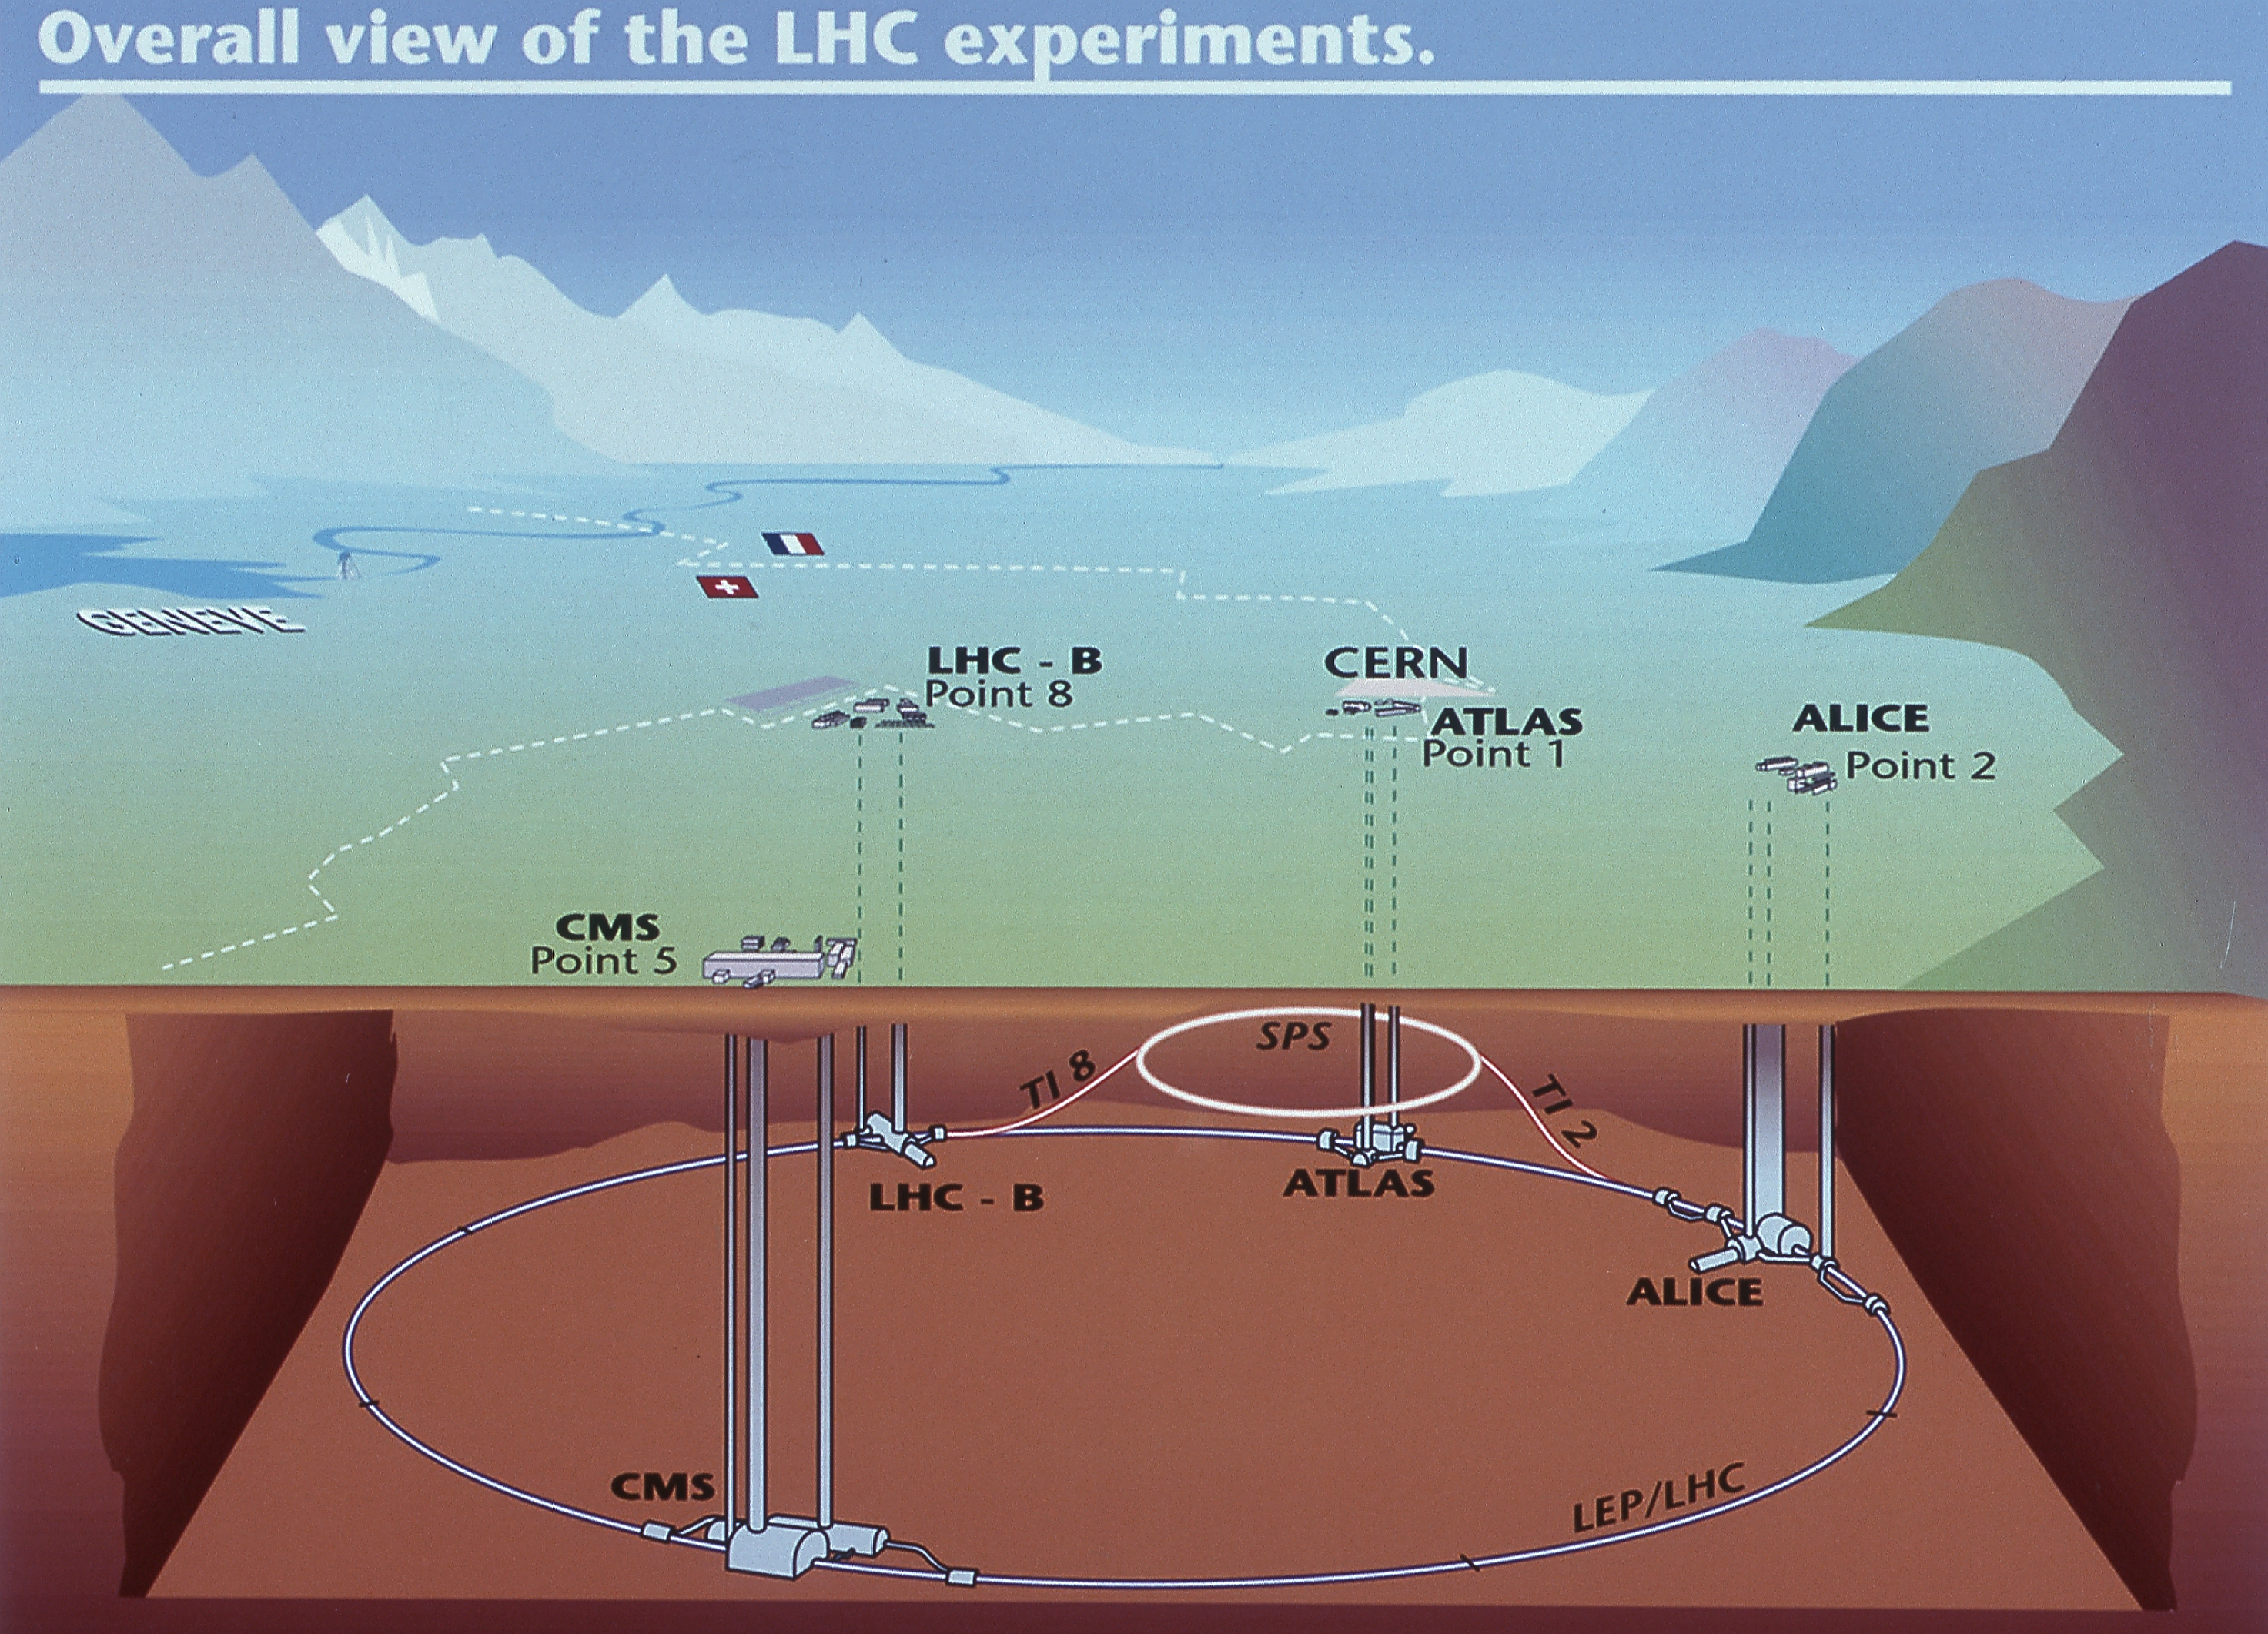
\includegraphics[width=0.8\textwidth]{Chapter2/LHC.jpg}
  \caption{This diagram shows the locations of the four main experiments (ALICE,
    ATLAS, CMS and LHCb) that take place at the LHC. Located between 50 m and
    150 m underground, huge caverns have been excavated to house the giant
    detectors. The Super Proton Synchotron (SPS), the final link in the
    pre-acceleration chain, and its connection tunnels to the LHC are also
    shown.  Figure from \cite{CERN:ATLASexperimentPictureswiki}  }
  \label{fig:LHC}
\end{figure}

LHC started to operate on November 23, 2009 and soon thereafter (March 30, 2010)
the proton-proton collisions achieved the center-of-mass energy $\sqrt{s} = 7
\TeV$, which is halve of the design energy of the machine. On April 5, 2012, the
machine started its successful $\sqrt{s} = 8 \TeV$ run.

Next to the proton-proton collisions first heavy-ion Pb-Pb collisions took place
in 2010 at a center of mass energy per pair of colliding nucleons $\sqrt{s} =
2.76 \TeV$. Proton-Pb collisions at $\sqrt{s} = 5.02 \TeV$ occurring on LHC
during 3 weeks of 2013 successfully demonstrated LHC capability to provide
asymmetric collisions.  

The first running period of the LHC, Run I, was very successful and resulted in
important discoveries including Higgs boson on July 4, 2012
\cite{HiggsDiscovery}.  The accelerator complex has been upgraded including its
experiments for two years and it is expected, the Run II will start in summer
2015 \cite{LHCFuture}. In Run II the center-of-mass energy of proton-proton
collisions will be raised up to $\sqrt{s} = 13 \TeV$ and beam crossing time will
be reduced from the current $50\,\text{ns}$ to $25\,\text{ns}$.

\subsection{The ATLAS Detector}

The ATLAS detector \cite{ATLAS} is a general-purpose detector surrounding one of
the interaction points of the LHC and with $\sim 100$ million of individual
electronic channels it is the most complicated instrument ever created having
one simple task: Record charged particle collisions up to the center-of-mass
energy per pair of colliding nucleons $\rts = 14 \TeV$. A detector overview is
shown in Figure~\ref{fig:ATLASfull}, where the main sub-detector systems can be
seen: the inner detector, used to reconstruct charged-particle tracks, the
electromagnetic calorimeters, the hadronic calorimeters, and the muon
spectrometer. 

\begin{figure}[p]
  \centering
  \begin{subfigure}[b]{0.9\textwidth}
    \includegraphics[width=\textwidth]{Chapter2/ATLAS.png}
    \caption{ATLAS detector}
    \label{fig:ATLASfull}
  \end{subfigure}
  ~
  \begin{subfigure}[b]{0.9\textwidth}
    \includegraphics[width=\textwidth]{Chapter2/ATLASinner.jpeg}
    \caption{Inner detector and calorimeter systems}
    \label{fig:ATLASinner}
  \end{subfigure}
  \caption{(a) an overview of the ATLAS detector 
           (b) detail on the inner detector and the calorimeters - the dominant
           sub-detector systems used in this thesis. Figures from
           \cite{CERNbook}.}
  \label{fig:ATLAS}
\end{figure}

ATLAS uses a right-handed coordinate system with its origin at the interaction
point in the center of the detector and the $z$ axis along the beam pipe. The
$x$ axis points from the interaction point to the center of the LHC ring, and
the $y$ axis points upward. Cylindrical coordinates $(r, \phi)$ are used in the
transverse plane, $\phi$ being the azimuthal angle around the beam pipe. Instead
of polar angle $\theta$ pseudorapidity $\eta$ is used throughout this thesis. For
event selection the rapidity $y$ plays an important role. In following
definitions of pseudorapidity $\eta$ and rapidity $y$, $E$ stands for the total
energy and $p$ for size of total momentum: 
\begin{eqnarray}
  \eta &= & - \frac{1}{2} \ln \left( \frac{p+p_z}{p-p_z} \right) = - \ln \left[
  \tan \left( \frac{\theta}{2} \right) \right], \\ y &= &- \frac{1}{2} \ln
  \left( \frac{E+p_z}{E-p_z} \right).	
\end{eqnarray}
The transverse momentum $\pt$ presents the component of momentum perpendicular
to the beam line.  

The main detector system relevant to this thesis is the ATLAS calorimeter,
which is emphasized in Figure~\ref{fig:ATLASinner}. The calorimeter is divided
into sub-detectors, providing overall coverage up to $|\eta| < 4.9$. The
electromagnetic calorimeter, covering region $|\eta| < 3.2$, is a
high-granularity sampling detector in which the active medium is liquid argon
(LAr) interspaced with layers of lead absorber. The hadronic calorimeters are
divided into three sections: a tile scintillator/steel calorimeter is used in
both the barrel ($|\eta| < 1.0$) and extended barrel cylinders ($0.8 < |\eta| <
1.7$) while the hadronic endcap ($1.5 < |\eta| < 3.2$) consists of LAr/copper
calorimeter modules. The forward calorimeter measures both electromagnetic and
hadronic energy in the range $3.2 < |\eta| < 4.9$ using LAr/copper and
LAr/tungsten modules. 

\section{Hadron Collision at LHC}

In this section the phenomenological description of proton-proton collisions
will be presented following picture in Figure \ref{fig:HardProcess} and
Reference about Monte Carlo event generators \cite{PDG}.

\begin{figure}[t]
  \centering
  \includegraphics[width=0.7\textwidth]{Chapter2/HardProcess.png}
  \caption{Schematic representation of a hard scattering proton-proton
    collision. Figure from \cite{HardProcess}}
  \label{fig:HardProcess}
\end{figure}

Two incoming protons can be understood as the bag of
partons. The collision alone is dominated by the interaction of two partons - one from
each of the colliding hadrons. These partons are called incoming partons and the
momentum transfer by their interaction is $Q \gg \Lambda$, so the perturbative
QCD can be used in the process of hard scattering. Only a small fraction of
collision energy has remained for the rest of the partons, which create the so
called underlying event - particles, which do not come from
the dominant QCD processes.

The perturbative QCD is used, while the remnants from collision of incoming
partons are in distance $<10^{-15}\,\text{m}$ from each other. There is for
example enough time for top quark to decay. When the distance between outgoing
partons becomes greater, the non-perturbative QCD has to be used to describe the
hadronisation - the process, by which a set of colored partons is
transformed into a set of colorless primary hadrons which may then decay
further. 

During the collision, the electric and color charges of partons interact
resulting in radiation of photons $q \rightarrow q\gamma$ and gluons $q
\rightarrow qg$. These processes are described be perturbative QCD and lead to
infrared and collinear divergences. However, infrared divergences can be
canceled by Kinoshita--Lee--Nauenberg theorem \cite{KLN1,KLN2}, so only
collinear divergences remain. There is no mechanism known up to date, which
would solve the problem with collinear divergence. However, observables
inclusive enough to be insensitive to processes that distinguish between
different numbers of partons are not affected by infrared divergences.
There is no possibility how to theoretically predict the energy of hardest
outgoing particle, but it is possible to predict the energy flow in a cone from
the point of scattering.

This is where the term jet comes to play. A jet can be naively seen as a group
of collimated particles generated by the hadronisation of a parton in the
scattering process and is the most important object used on hadron colliders for
analysis of QCD processes.

\section{Jet Algorithms}

Jet algorithm is a generic "recipe" which takes a set of particles (or other
objects with defined
four-momenta) and returns jets created from them. That recipe usually involves a
set of parameters which together with the recipe fully specify the jet
definition. Following the remarks at the end of the previous section, jet
algorithms should fulfill following conditions 
\begin{enumerate}
  \item Infrared safety - the presence of additional soft particles between two
    particles belonging to the same jet should not affect the recombination of
    these particles into a jet.
  \item Collinear safety - jet reconstruction should not depend on fact, if
    transverse momentum is carried by one particle, or if a particle is split
    into two collinear particles.
\end{enumerate}

Principals of two jet algorithms are described here - fixed cone algorithm and
$k_t$ algorithm. First of these algorithms is more illustrative, the second one
is used in ATLAS. Detailed description as well as other jet algorithms can be
found in \cite{ATLASmain}. After definitions of jet algorithms it is shortly
described, how the objects (not necessary particles) with defined four-momenta
are constructed from the signal observed on the ATLAS detector.

\subsection{Fixed cone algorithm}

The first step of this algorithm is to order all input objects (reconstructed
detector objects with four-momentum representation) in decreasing order in
transverse momentum $\pt$. If the object with the highest $\pt$ is above the
seed threshold, all objects within a cone in pseudorapidity $\eta$ and azimuth
$\phi$ with $\Delta R = \sqrt{\Delta \eta^2 + \Delta \phi^2} < R_{cone}$, where
$R_{cone}$ is the fixed cone radius, are combined together. A new direction is
calculated from the four-momenta inside the initial cone and a new cone is
centered around it. Objects are then recollected in this new cone and again the
direction is updated. This process continues until the direction of the cone
does not change anymore after recombination, at which point the cone is
considered stable and is called a jet. At this point, the next seed is taken
from the input list and a new cone jet is formed with the same iterative
procedure. This continues until no more seeds are available. 

The jets found this way can share some constituents. This algorithm is both not
infrared safe (Figure \ref{fig:IRsafety}) and not collinear safe (Figure
\ref{fig:ColSafety}).

\begin{figure}[t]
  \centering
  \begin{subfigure}[b]{0.65\textwidth}
    \includegraphics[width=\textwidth]{Chapter2/IRsafety.png}
    \caption{Infrared unsafety}
    \label{fig:IRsafety}
  \end{subfigure}
  ~
  \begin{subfigure}[b]{0.6\textwidth}
    \includegraphics[width=\textwidth]{Chapter2/ColSafety.png}
    \caption{Collinear unsafety}
    \label{fig:ColSafety}
  \end{subfigure}
  \caption{Illustration of (a) infrared unsafety and (b) collinear unsafety
    of fixed cone jet algorithm.
    Figures from \cite{JetTheoreticalPictures}.}
  \label{fig:JetIRCOLsafety}
\end{figure}

Parameters used by fixed cone algorithm are a seed threshold of $\pt > 1 \GeV$,
and a narrow ($R_{cone} = 0.4$) or a wide cone jet ($R_{cone} = 0.7$) option.

\subsection{$k_t$ algorithms}

In this class of algorithms all pairs $(i,j)$ of input objects are analyzed with
respect to their relative transverse momentum squared, defined by 

\begin{equation}
	d_{ij} = \min{\left( p_{T,i}^{2p} , p_{T,j}^{2p} \right)} \frac{\Delta R_{ij}^2}{R^2}
\end{equation}
and the squared $\pt$ of object $i$ relative to the beam axis

\begin{equation}
	d_i = p_{T,i}^{2p}.
\end{equation}
Here $\Delta R_{ij}^2 = (y_i - y_j)^2 + (\phi_i - \phi_j)^2$ and $p_{T,i}$,
$y_i$ and $\phi_i$ are respectively the transverse momentum, rapidity and
azimuth of particle $i$. In addition to the radius parameter $R$, parameter $p$
was added to split $k_t$~algorithms into three categories.  
\begin{itemize}
	\item $p = 1$ $k_t$ algorithm,
	\item $p = 0$ Cambridge/Aachen algorithm,
	\item $p = -1$ anti-$k_t$ jet-clustering algorithm.
\end{itemize}
The differences between these algorithms are detailed described
in~\cite{ANTIKT}. Recombination of calorimeter signal towers (see Section
\ref{sse:CalorimeterJets}) in jets is for $k_t$ and anti-$k_t$ algorithms shown
at Figure 

\begin{figure}[t]
  \centering
  \includegraphics[width=\textwidth]{Chapter2/JetRecombination.png}
  \caption{Illustration of $k_t$ and anti-$k_t$ jet algorithms with $R=1$ for
    calorimeter signal towers in azimuth $\Phi$ and pseudorapidity $y$. Towers of
    the same color were recombined to one jet. Figure from
    \cite{JetTheoreticalPictures}} 
  \label{fig:JetRecombination}
\end{figure}

These algorithms first find the minimum $d_{min}$ of all $d_{ij}$ and $d_i$. If
$d_{min}$ is in $d_{ij}$'s, the corresponding objects $i$ and $j$ are combined
into a new object $k$ using four-momentum recombination. Both objects $i$ and
$j$ are removed from the list, and the new object $k$ is added to it. If
$d_{min}$ is in $d_i$'s, the object $i$ is considered to be a jet by itself and
removed from the list.

This means that all original input objects end up to be either part of a jet or
to be jets by themselves. Contrary to the cone algorithm described earlier, no
objects are shared between jets and the procedure is both infrared and collinear
safe.

ATLAS uses anti-$k_t$ algorithm with $R=0.4$ for narrow and $R=0.6$ for wide
jets.

\subsection{Calorimeter jets}
\label{sse:CalorimeterJets}

The most important detectors for jet reconstruction are the ATLAS calorimeters.
The ATLAS calorimeter system has about 200,000 individual cells of various sizes
and with different readout technologies and cell geometries. For jet finding it
is necessary to first combine these cell signals into larger signal object with
physically meaningful four-momenta. The two concepts available are calorimeter
signal towers and topological cell clusters.

In the case of calorimeter signal towers, the cells are projected onto a fixed
grid in pseudorapidity $\eta$ and azimuth $\phi$. The tower bin size is $\Delta
\eta \times \Delta \phi = 0.1 \times 0.1$ in the whole acceptance region of the
calorimeters, i.e. in $|\eta| < 5$ and $- \pi < \phi < \pi$ with approximately 
$100 \times 64 = 6,400$ towers in total.

The alternative representation of the calorimenter signals for jet
reconstruction are topological cell clusters, which are basically an attempt to
reconstruct three-dimensional "energy blobs" representing the showers developing
for each particle entering the calorimeter. The clustering starts with seed
cells with a signal-to-noise ratio, or signal significance $\Gamma = E_{cell} /
\sigma_{noise,cell}$, above a certain threshold $S$, i.e. $|\Gamma| > S = 4$.
All directly neighbouring cells of these seed cells, in all three dimensions,
are collected into the cluster. Neighbours of neighbours are considered for
those added cells which have $\Gamma$ above a certain secondary threshold $N$
($|\Gamma| > N = 2$). Finally, a ring of guard cells with signal significances
above a basic threshold $|\Gamma| > P = 0$ is added to the cluster. After the
initial clusters are formed, they are analyzed for local signal maximums by a
splitting algorithm, and split between those maximums.

\chapter{Data Analysis}





\begin{table}
  \centering
  \begin{tabular}{|c|rcr|c|c|c|}
    \hline 
     JZXW & \multicolumn{3}{|c|}{$\pt$ range (GeV)} & Cross-section (fb) & Filter Efficiency & \# envents  \\ 
    \hline
    \hline
		 JZ0W &     0 & - &    20 & 7.8420e+13 & 9.7193e-01 & 3498000 \\ 
    \hline
		 JZ1W &    20 & - &    80 & 7.8420e+13 & 2.7903e-04 & 2998000 \\
    \hline
		 JZ2W &    80 & - &   200 & 5.7312e+10 & 5.2261e-03 & 500000  \\
    \hline
		 JZ3W &   200 & - &   500 & 1.4478e+09 & 1.8068e-03 & 499500  \\
    \hline
		 JZ4W &   500 & - &  1000 & 2.3093e+07 & 1.3276e-03 & 477000  \\
    \hline
		 JZ5W &  1000 & - &  1500 & 2.3793e+05 & 5.0449e-03 & 499000  \\
    \hline
		 JZ6W &  1500 & - &  2000 & 5.4279e+03 & 1.3886e-02 & 493500  \\
    \hline
		 JZ7W &  2000 & + &       & 9.4172e+02 & 6.7141e-02 & 497000  \\
    \hline 
  \end{tabular}
  \caption{The cross-sections, filter efficiency and number of events for the JZXW samples which differ in the leading truth jet $\pt$.}
  \label{tab:JZXW}
\end{table}





\begin{landscape} 
\begin{table}
  \centering
  \begin{tabular}{|c|c|>{\bfseries}c|c|c|c|c|c|c|c|c|}
    \hline
     \multicolumn{2}{|c|}{\# jets}  & ALL      & JZ0W     & JZ1W     & JZ2W     & JZ3W     & JZ4W     & JZ5W     & JZ6W     & JZ7W     \\
    \hline                                                              
    \hline                                                              
     \multicolumn{2}{|c|}{Signal}   & 1.10e+08 & 3.22e+07 & 3.59e+07 & 6.67e+06 & 7.07e+06 & 6.28e+06 & 7.29e+06 & 7.13e+06 & 7.11e+06 \\
    \hline                                                              
     \multicolumn{2}{|c|}{Truth}    & 7.22e+07 & 3.15e+06 & 3.00e+07 & 6.17e+06 & 6.91e+06 & 6.20e+06 & 6.98e+06 & 6.53e+06 & 6.25e+06 \\
    \hline                                                              
    \hline                                                              
    \multirow{4}{*}{CutPt}          & \multirow{2}{*}{Signal}   & 1.32e+07 & 5.45e+06 & 4.38e+06 & 6.50e+05 & 5.87e+05 & 4.76e+05 & 5.48e+05 & 5.52e+05 & 5.63e+05 \\
                                    &                           & 12.1 \%  & 17.0 \%  & 12.2 \%  & 9.7 \%   & 8.3 \%   & 7.6 \%   & 7.5 \%   & 7.7 \%   & 7.9 \%   \\
    \cline{2-11}                                                                 
                                    & \multirow{2}{*}{Truth}    & 4.67e+07 & 3.11e+06 & 2.20e+07 & 3.86e+06 & 4.00e+06 & 3.42e+06 & 3.74e+06 & 3.43e+06 & 3.23e+06 \\
                                    &                           & 64.7 \%  & 98.7 \%  & 73.1 \%  & 62.6 \%  & 57.8 \%  & 55.1 \%  & 53.6 \%  & 52.5 \%  & 51.6 \%  \\
    \hline                                                              
    \hline                                                              
    \multirow{4}{*}{Cuty}           & \multirow{2}{*}{Signal}   & 2.46e+06 & 8.02e+05 & 9.54e+05 & 1.42e+05 & 1.28e+05 & 1.03e+05 & 1.16e+05 & 1.10e+05 & 1.08e+05 \\
                                    &                           & 2.2 \%   & 2.5 \%   & 2.7 \%   & 2.1 \%   & 1.8 \%   & 1.6 \%   & 1.6 \%   & 1.5 \%   & 1.5 \%   \\
    \cline{2-11}                                                                                    
                                    & \multirow{2}{*}{Truth}    & 5.03e+05 & 3.14e+03 & 3.19e+05 & 4.54e+04 & 3.79e+04 & 2.88e+04 & 2.78e+04 & 2.22e+04 & 1.83e+04 \\
                                    &                           & 0.7 \%   & 0.1 \%   & 1.1 \%   & 0.7 \%   & 0.5 \%   & 0.5 \%   & 0.4 \%   & 0.3 \%   & 0.3 \%   \\
    \hline                                                              
    \hline                                                              
    \multirow{4}{*}{Cut0jet}        & \multirow{2}{*}{Signal}   & 2.62e+07 & 2.56e+07 & 5.49e+05 & 0.00e+00 & 0.00e+00 & 0.00e+00 & 0.00e+00 & 0.00e+00 & 0.00e+00 \\
                                    &                           & 23.9 \%  & 79.6 \%  & 1.5 \%   & 0.0 \%   & 0.0 \%   & 0.0 \%   & 0.0 \%   & 0.0 \%   & 0.0 \%   \\
    \cline{2-11}                                                                                    
                                    & \multirow{2}{*}{Truth}    & 0.00e+00 & 0.00e+00 & 0.00e+00 & 0.00e+00 & 0.00e+00 & 0.00e+00 & 0.00e+00 & 0.00e+00 & 0.00e+00 \\
                                    &                           & 0.0 \%   & 0.0 \%   & 0.0 \%   & 0.0 \%   & 0.0 \%   & 0.0 \%   & 0.0 \%   & 0.0 \%   & 0.0 \%   \\
    \hline                                                              
    \hline                                                              
    \multirow{4}{*}{CutLR}          & \multirow{2}{*}{Signal}   & 3.64e+06 & 2.27e+05 & 3.37e+06 & 2.99e+04 & 7.07e+03 & 2.33e+03 & 1.63e+03 & 7.14e+02 & 6.31e+02 \\
                                    &                           & 3.3 \%   & 0.7 \%   & 9.4 \%   & 0.4 \%   & 0.1 \%   & 0.0 \%   & 0.0 \%   & 0.0 \%   & 0.0 \%   \\
    \cline{2-11}                                                                                    
                                    & \multirow{2}{*}{Truth}    & 5.21e+05 & 2.15e+04 & 4.74e+05 & 1.82e+04 & 4.45e+03 & 1.33e+03 & 9.03e+02 & 4.37e+02 & 2.78e+02 \\
                                    &                           & 0.7 \%   & 0.7 \%   & 1.6 \%   & 0.3 \%   & 0.1 \%   & 0.0 \%   & 0.0 \%   & 0.0 \%   & 0.0 \%   \\
    \hline                                                              
    \hline                                                              
    \multirow{4}{*}{Matched}        & \multirow{2}{*}{Signal}   & 2.13e+07 & 7.95e+03 & 5.99e+06 & 1.95e+06 & 2.54e+06 & 2.46e+06 & 2.88e+06 & 2.78e+06 & 2.72e+06 \\
                                    &                           & 19.5 \%  & 0.0 \%   & 16.7 \%  & 29.3 \%  & 36.0 \%  & 39.1 \%  & 39.5 \%  & 38.9 \%  & 38.2 \%  \\
    \cline{2-11}                                                                                    
                                    & \multirow{2}{*}{Truth}    & 2.13e+07 & 7.95e+03 & 5.99e+06 & 1.95e+06 & 2.54e+06 & 2.46e+06 & 2.88e+06 & 2.78e+06 & 2.72e+06 \\
                                    &                           & 29.5 \%  & 0.3 \%   & 19.9 \%  & 31.7 \%  & 36.8 \%  & 39.6 \%  & 41.3 \%  & 42.5 \%  & 43.5 \%  \\
    \hline                                                              
    \hline                                                              
    \multirow{4}{*}{Unmatched}      & \multirow{2}{*}{Signal}   & 4.28e+07 & 6.15e+04 & 2.06e+07 & 3.89e+06 & 3.81e+06 & 3.24e+06 & 3.75e+06 & 3.69e+06 & 3.72e+06 \\
                                    &                           & 39.0 \%  & 0.2 \%   & 57.5 \%  & 58.4 \%  & 53.8 \%  & 51.6 \%  & 51.4 \%  & 51.8 \%  & 52.3 \%  \\
    \cline{2-11}                                                                                    
                                    & \multirow{2}{*}{Truth}    & 3.14e+06 & 7.51e+03 & 1.30e+06 & 2.89e+05 & 3.29e+05 & 2.95e+05 & 3.29e+05 & 3.03e+05 & 2.88e+05 \\
                                    &                           & 4.4 \%   & 0.2 \%   & 4.3 \%   & 4.7 \%   & 4.8 \%   & 4.8 \%   & 4.7 \%   & 4.6 \%   & 4.6 \%   \\
    \hline
  \end{tabular}
  \caption{Cut and matching efficiency.}
  \label{tab:CutAndMatchingEfficiency}
\end{table} 
\end{landscape}


\chapter*{Conclusion}
\addcontentsline{toc}{chapter}{Conclusion}

This thesis deals with the measurement of the inclusive jet double differential
cross section in $\pt$ and rapidity. Inclusive jets are dominant objects created
by the ultrarelativistic collisions at Large Hadron Collider (LHC) with $\pt$
covering range from a few $\GeV$ to a few $\TeV$. Nowhere is the increase in the
center-of-mass energy appreciated as is in the case of inclusive jets as it can
be seen from figure ?.  According to the preliminary analysis, the $pp$
collision in LHC Run II with the center-of-mass energy $\sqrt{s} = 13\TeV$ could
create a thousands of jets with $1\TeV < \pt < 4\TeV$.

Inclusive jets are theoretically straightforward and hence powerful test of
perturbative Quantum chromodynamics (pQCD) and with wide range of 
momentum transfers, the inclusive jet cross section is sensitive to the
properties of the running coupling constant $\alpha_S$.  Momentum transfers in
orders of $\sim 1 \TeV$ will probe the structure of proton at small distance
scales $\lambda \sim 1 / \pt \sim \TeV^{-1} \sim 10^{-19} \, \text{m}$ and will
contribute to our understanding of the proton structure (parton distribution
functions (PDF)). If there is new physics at these scales (such as the
structure of quark), the inclusive jets may reveal it.

After an introduction, thesis begins with a brief description of the Quantum
Chromodynamics (QCD) as one of the parts of the Standard Model (SM) following
its historical development during which description the key concepts of QCD are
introduced.  These include the PDFs, running coupling constant $\alpha_S$ and
asymptotic freedom phenomenons, leading to splitting QCD into perturbative and
non-perturbative regions. 

LHC with the ATLAS detector are described in the second chapter in which the key
concept of this thesis - the jet - is defined. This include the description of
jet algorithms with emphasize on anti-$k_t$ jet algorithm relevant for this
thesis and the procedure which must be done to detector recorded signal
could be compared with the theoretical predictions of QCD leading to inevitable
definitions of jet calibration and unfolding procedures. 

Last chapter describes the analysis done in this thesis.



%================================================================================
% Appendices
%================================================================================

\begin{appendices}

\chapter{Cut and Match Results}
\label{App:CutAndMatchingResults}

\newpage 

\section{Cut Results}
\label{sec:CutResults}

\begin{figure}[H]
  \centering
  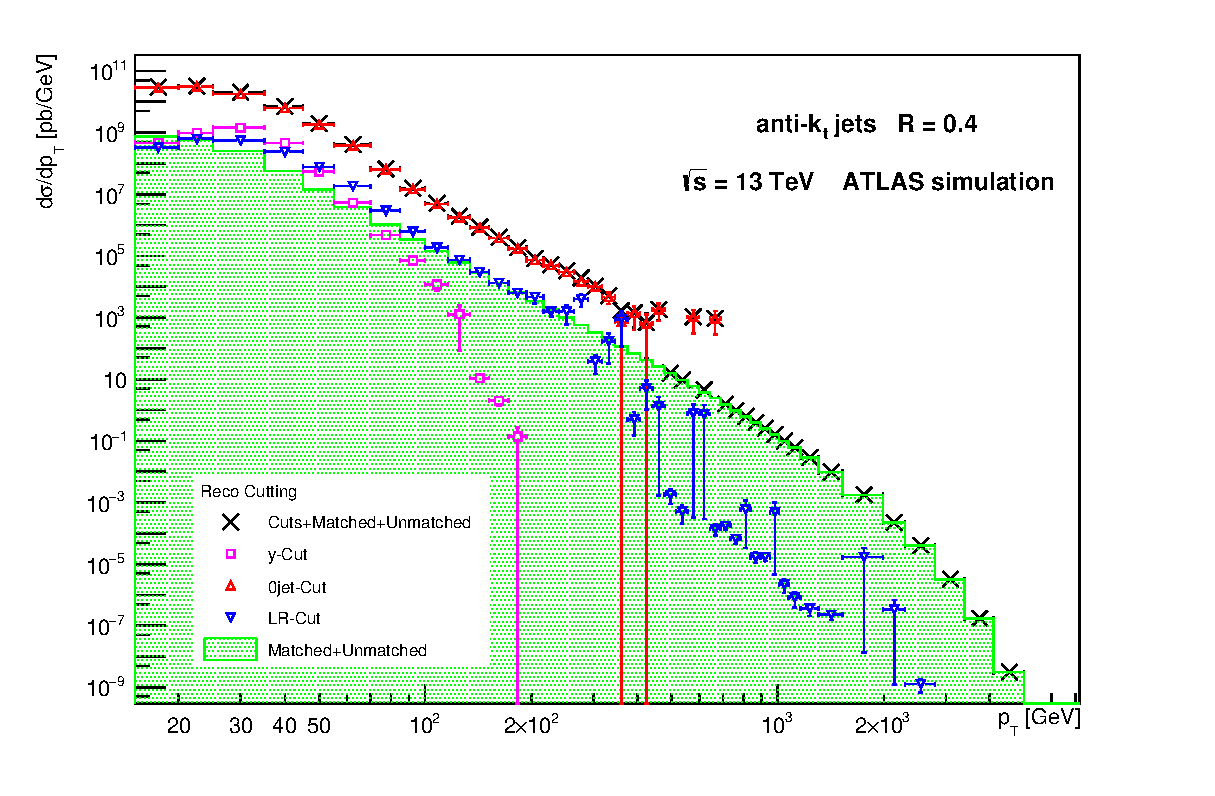
\includegraphics[width=\textwidth]{Chapter3/SignalCutting.eps}
  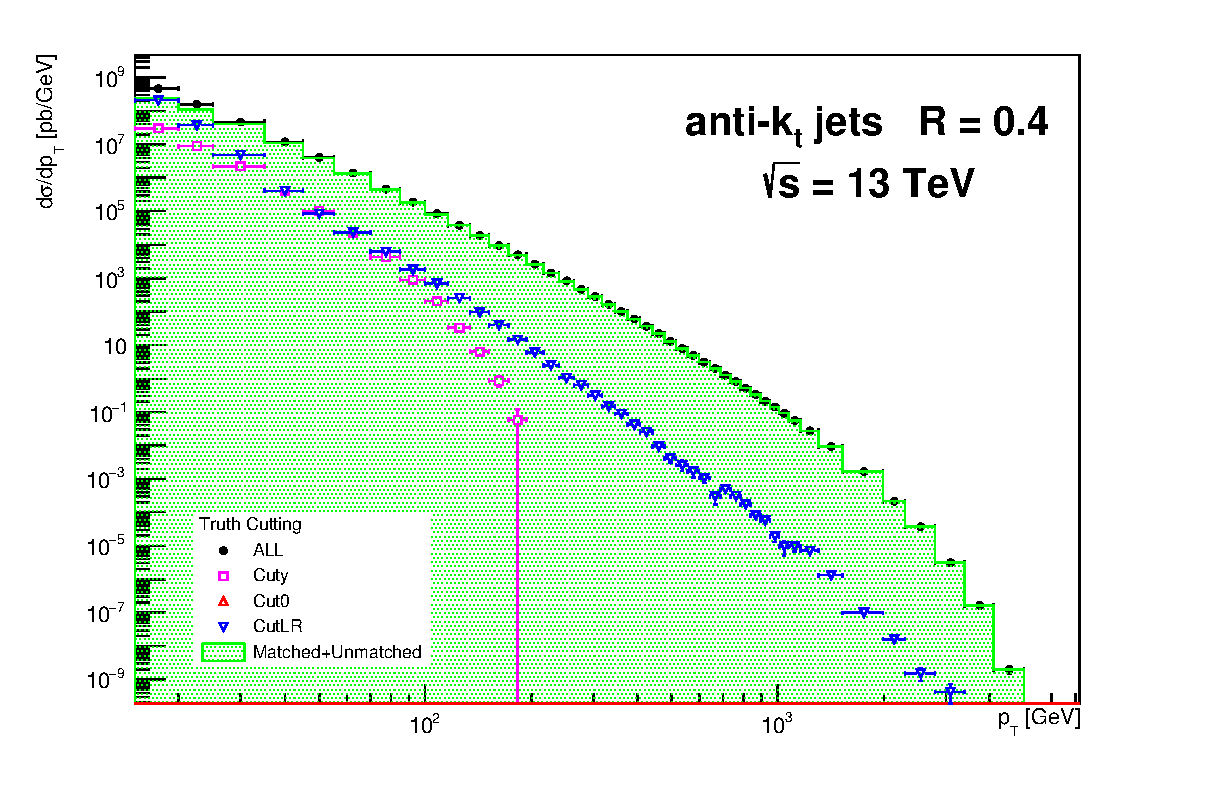
\includegraphics[width=\textwidth]{Chapter3/TruthCutting.eps}
  \caption{Impact of 4 cuts defined in Section \ref{SubSec:JetCuts} on
  differential cross section in $\pt$ of signal jets (top) and truth jets
  (bottom). Black dots represent the original uncutted spectrum, green area then
  these jets, which survived all four cutoffs.}
  \label{fig:Cutting}
\end{figure}

\section{Match Results}
\label{sed:MatchResults}

\begin{figure}[H]
  \centering
  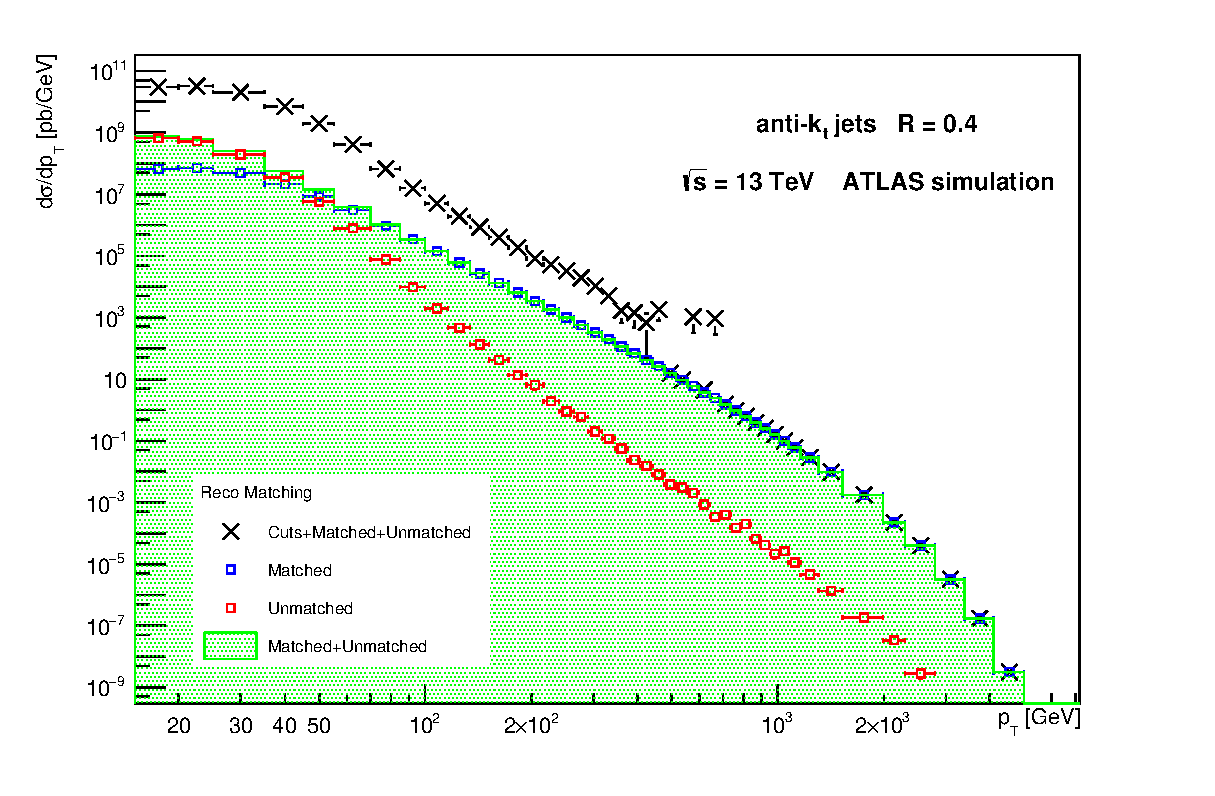
\includegraphics[width=\textwidth]{Chapter3/SignalMatching.eps}
  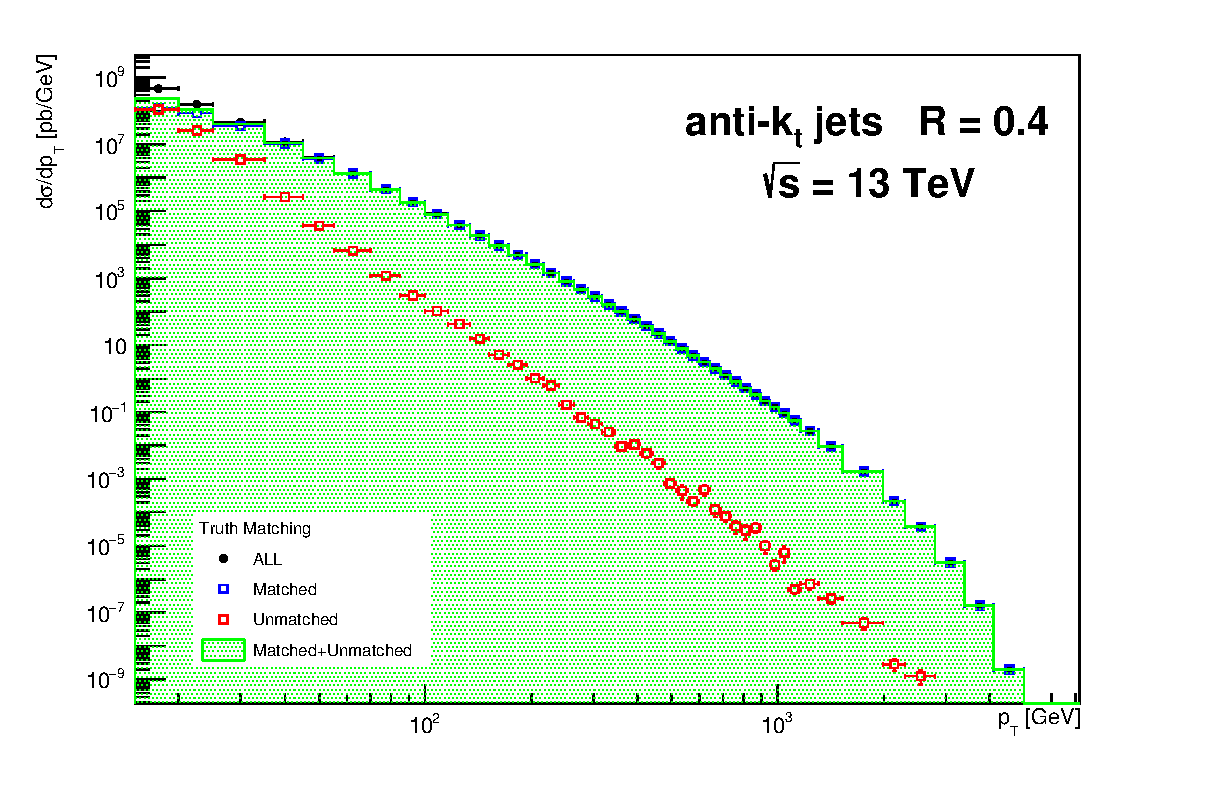
\includegraphics[width=\textwidth]{Chapter3/TruthMatching.eps}
  \caption{Results of matching procedure described in Section
  \ref{SubSec:JetMatching} demonstrated on differential cross section in $\pt$ of
  signal (top) and truth (bottom) jets. Black dots represent the original
  uncutted spectrum. The contribution of matched and unmatched jets to
  green area representing all jets which survived cutoffs is shown.}
  \label{fig:Matching}
\end{figure}

\section{Truth and Reco $\pt$ Spectra}
\label{sec:TruthAndRecoSpectra}

\begin{figure}[H]
  \centering
  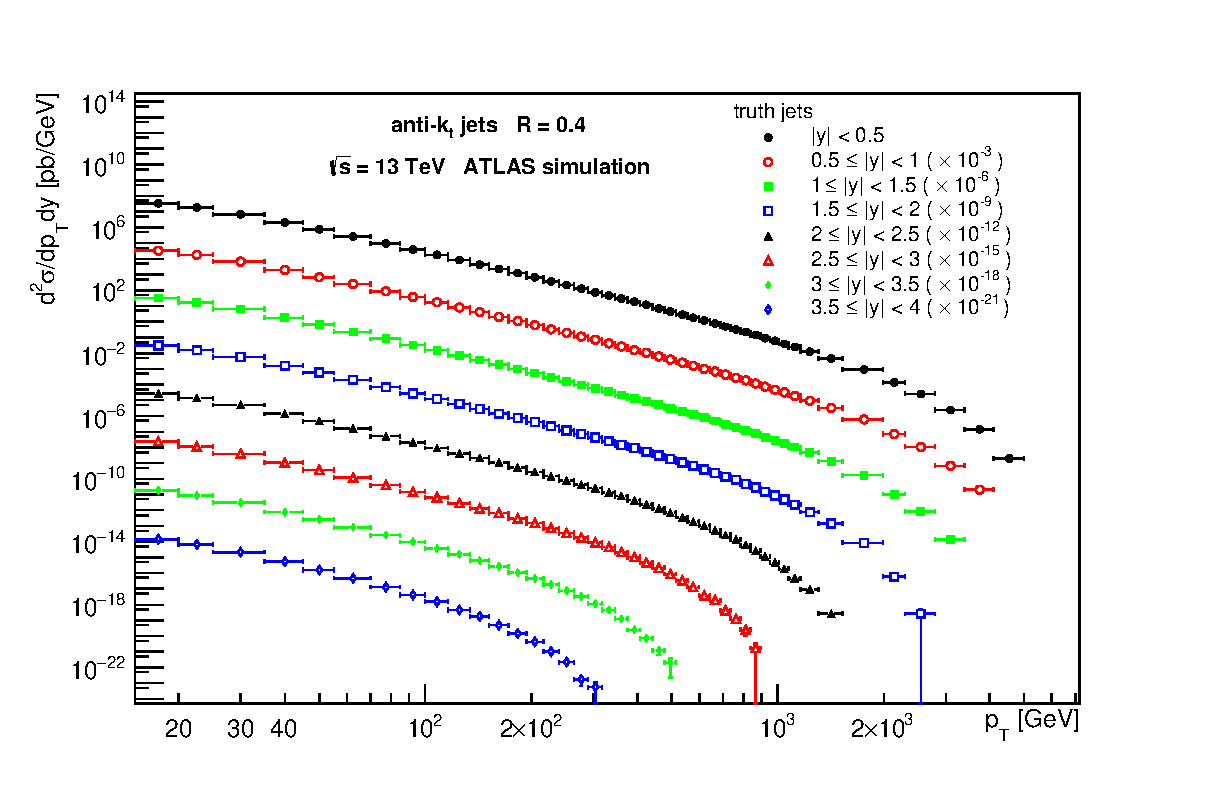
\includegraphics[width=\textwidth]{Chapter3/ptTruthAllRapidityBins.eps}
  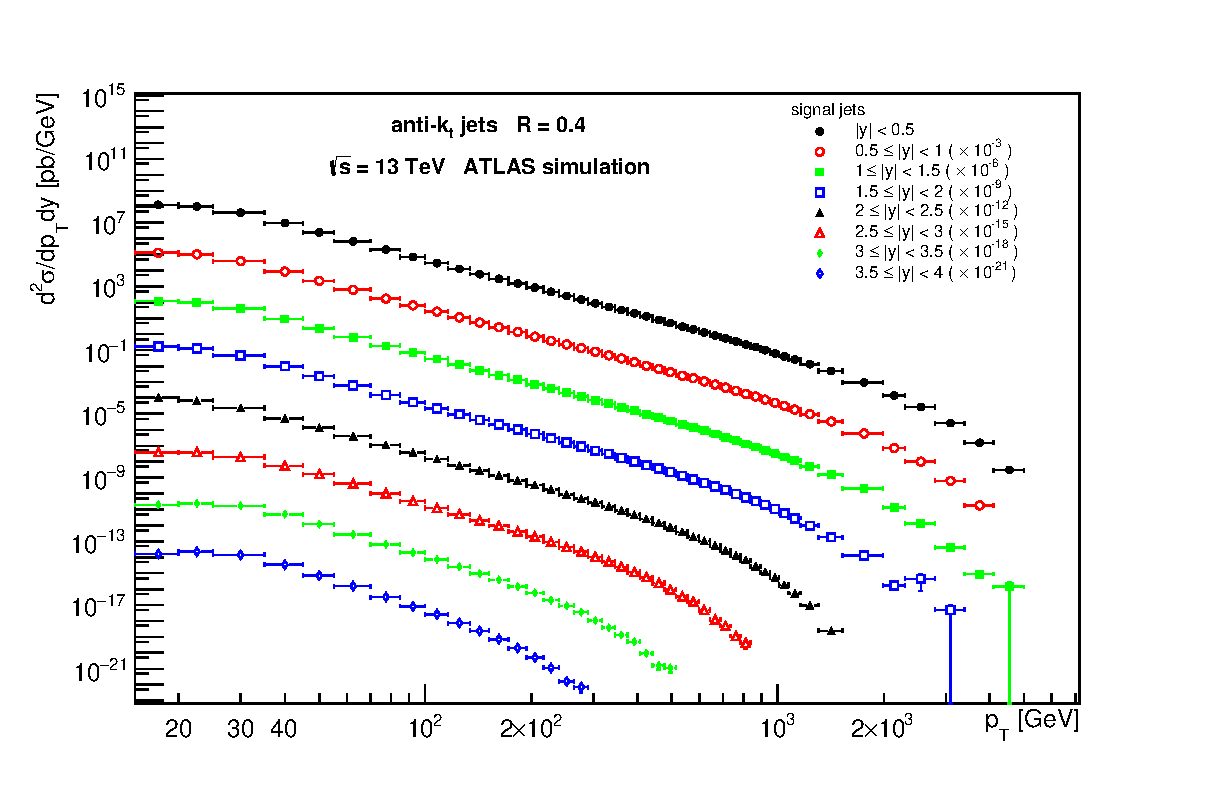
\includegraphics[width=\textwidth]{Chapter3/ptSignalAllRapidityBins.eps}
  \caption{Inclusive jet cross section of truth (top) and reco (bottom) jets as
    the function of jet $\pt$ and rapidity. For the convenience the cross
    sections for different rapidity bins are multiplied by the factor indicated
    in the legend. Jets were identified with anti-$k_t$ jet algorithm with
    $R=0.4$.}
  \label{fig:ptSpectraMasacreEverythingFuck}
\end{figure}


\begin{landscape} 
\begin{table}
  \small
  \centering
  \begin{tabular}{|c|c|>{\bfseries}c|c|c|c|c|c|c|c|c|}
    \hline
     \multicolumn{2}{|c|}{\# jets}  & ALL      & JZ0W     & JZ1W     & JZ2W     & JZ3W     & JZ4W     & JZ5W     & JZ6W     & JZ7W     \\
    \hline                                                              
    \hline                                                              
     \multicolumn{2}{|c|}{Signal}                               & 1.09e+08 & 3.11e+07 & 3.59e+07 & 6.67e+06 & 7.07e+06 & 6.28e+06 & 7.29e+06 & 7.13e+06 & 7.11e+06 \\
    \hline                                                                                          
     \multicolumn{2}{|c|}{Truth}                                & 7.28e+07 & 3.04e+06 & 3.00e+07 & 6.17e+06 & 6.91e+06 & 6.20e+06 & 6.98e+06 & 6.53e+06 & 6.25e+06 \\
    \hline                                                                                      
    \hline                                                                                      
    \multirow{4}{*}{CutPt}          & \multirow{2}{*}{Signal}   & 9.36e+06 & 3.74e+06 & 3.13e+06 & 6.50e+05 & 5.87e+05 & 4.76e+05 & 5.48e+05 & 5.52e+05 & 5.63e+05 \\
                                    &                           & 8.6 \%   & 12.0 \%  & 8.7 \%   & 9.7 \%   & 8.3 \%   & 7.6 \%   & 7.5 \%   & 7.7 \%   & 7.9 \%   \\
    \cline{2-11}                                                                                
                                    & \multirow{2}{*}{Truth}    & 4.70e+07 & 3.00e+06 & 2.20e+07 & 3.86e+06 & 4.00e+06 & 3.42e+06 & 3.74e+06 & 3.43e+06 & 3.23e+06 \\
                                    &                           & 64.6 \%  & 98.7 \%  & 73.1 \%  & 62.6 \%  & 57.8 \%  & 55.1 \%  & 53.6 \%  & 52.5 \%  & 51.6 \%  \\
    \hline                                                                                      
    \hline                                                                                      
    \multirow{4}{*}{Cuty}           & \multirow{2}{*}{Signal}   & 3.43e+06 & 1.19e+06 & 1.29e+06 & 1.42e+05 & 1.28e+05 & 1.03e+05 & 1.16e+05 & 1.10e+05 & 1.08e+05 \\
                                    &                           & 3.1 \%   & 3.8 \%   & 3.6 \%   & 2.1 \%   & 1.8 \%   & 1.6 \%   & 1.6 \%   & 1.5 \%   & 1.5 \%   \\
    \cline{2-11}                                                                                    
                                    & \multirow{2}{*}{Truth}    & 5.06e+05 & 3.04e+03 & 3.19e+05 & 4.54e+04 & 3.79e+04 & 2.88e+04 & 2.78e+04 & 2.22e+04 & 1.83e+04 \\
                                    &                           & 0.7 \%   & 0.1 \%   & 1.1 \%   & 0.7 \%   & 0.5 \%   & 0.5 \%   & 0.4 \%   & 0.3 \%   & 0.3 \%   \\
    \hline                                                                                      
    \hline                                                                                      
    \multirow{4}{*}{Cut0jet}        & \multirow{2}{*}{Signal}   & 2.64e+07 & 2.59e+07 & 5.70e+05 & 0.00e+00 & 0.00e+00 & 0.00e+00 & 0.00e+00 & 0.00e+00 & 0.00e+00 \\
                                    &                           & 24.2 \%  & 83.2 \%  & 1.6 \%   & 0.0 \%   & 0.0 \%   & 0.0 \%   & 0.0 \%   & 0.0 \%   & 0.0 \%   \\
    \cline{2-11}                                                                                    
                                    & \multirow{2}{*}{Truth}    & 0.00e+00 & 0.00e+00 & 0.00e+00 & 0.00e+00 & 0.00e+00 & 0.00e+00 & 0.00e+00 & 0.00e+00 & 0.00e+00 \\
                                    &                           & 0.0 \%   & 0.0 \%   & 0.0 \%   & 0.0 \%   & 0.0 \%   & 0.0 \%   & 0.0 \%   & 0.0 \%   & 0.0 \%   \\
    \hline                                                                                      
    \hline                                                                                      
    \multirow{4}{*}{CutLR}          & \multirow{2}{*}{Signal}   & 4.09e+06 & 2.38e+05 & 3.82e+06 & 2.99e+04 & 7.07e+03 & 2.33e+03 & 1.63e+03 & 7.14e+02 & 6.31e+02 \\
                                    &                           & 3.7 \%   & 0.8 \%   & 10.6 \%  & 0.4 \%   & 0.1 \%   & 0.0 \%   & 0.0 \%   & 0.0 \%   & 0.0 \%   \\
    \cline{2-11}                                                                                    
                                    & \multirow{2}{*}{Truth}    & 5.40e+05 & 2.19e+04 & 4.96e+05 & 1.82e+04 & 4.45e+03 & 1.33e+03 & 9.03e+02 & 4.37e+02 & 2.78e+02 \\
                                    &                           & 0.7 \%   & 0.7 \%   & 1.7 \%   & 0.3 \%   & 0.1 \%   & 0.0 \%   & 0.0 \%   & 0.0 \%   & 0.0 \%   \\
    \hline                                                                                      
    \hline                                                                                      
    \multirow{4}{*}{Matched}        & \multirow{2}{*}{Signal}   & 2.17e+07 & 7.62e+03 & 6.03e+06 & 1.95e+06 & 2.54e+06 & 2.46e+06 & 2.88e+06 & 2.78e+06 & 2.72e+06 \\
                                    &                           & 19.8 \%  & 0.0 \%   & 16.8 \%  & 29.3 \%  & 36.0 \%  & 39.1 \%  & 39.5 \%  & 38.9 \%  & 38.2 \%  \\
    \cline{2-11}                                                                                    
                                    & \multirow{2}{*}{Truth}    & 2.17e+07 & 7.62e+03 & 6.03e+06 & 1.95e+06 & 2.54e+06 & 2.46e+06 & 2.88e+06 & 2.78e+06 & 2.72e+06 \\
                                    &                           & 29.8 \%  & 0.3 \%   & 20.1 \%  & 31.7 \%  & 36.8 \%  & 39.6 \%  & 41.3 \%  & 42.5 \%  & 43.5 \%  \\
    \hline                                                                                      
    \hline                                                                                      
    \multirow{4}{*}{Unmatched}      & \multirow{2}{*}{Signal}   & 4.42e+07 & 5.36e+04 & 2.10e+07 & 3.89e+06 & 3.81e+06 & 3.24e+06 & 3.75e+06 & 3.69e+06 & 3.72e+06 \\
                                    &                           & 40.5 \%  & 0.2 \%   & 58.6 \%  & 58.4 \%  & 53.8 \%  & 51.6 \%  & 51.4 \%  & 51.8 \%  & 52.3 \%  \\
    \cline{2-11}                                                                                    
                                    & \multirow{2}{*}{Truth}    & 3.07e+06 & 6.18e+03 & 1.25e+06 & 2.89e+05 & 3.29e+05 & 2.95e+05 & 3.29e+05 & 3.03e+05 & 2.88e+05 \\
                                    &                           & 4.2 \%   & 0.2 \%   & 4.2 \%   & 4.7 \%   & 4.8 \%   & 4.8 \%   & 4.7 \%   & 4.6 \%   & 4.6 \%   \\
    \hline
  \end{tabular}
  \caption{Statistics for matching and cutting procedures described in Sections
    \ref{SubSec:JetCuts} and \ref{SubSec:JetMatching} displayed for all jets and for
    individual JZXW samples defined in Table \ref{tab:JZXW}. At the top, there is
    number of initial signal and truth jets respectively. For each cut, there is
    shown the number of jets, which were killed by it, and their relative number
    according to the original number of signal or truth jets respectively.
    Last two lines show the statistics of matching procedure including number of
    jets which were (un)matched.}
  \label{tab:CutAndMatchingEfficiency}
\end{table} 
\end{landscape}

\chapter{Unfolding}
\label{App:UnfoldingResults}

\section{Matching Efficiency}
\label{sec:MatchingEfficiency}

\begin{figure}[H]
  \centering
  \includegraphics[width=0.49\textwidth]{{Chapter3/MatchEffSimpe2DSignal|abs(y)|0-0.5Compare}.eps}
  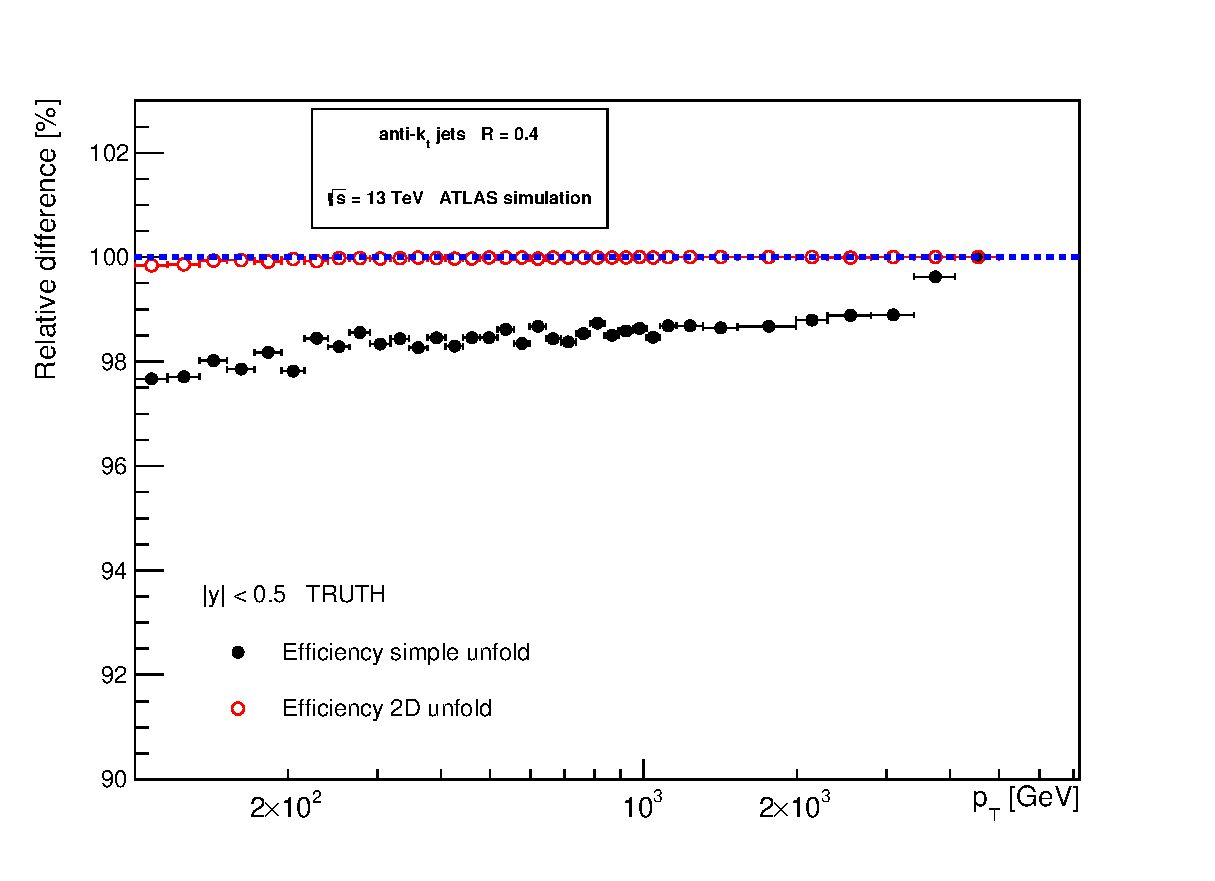
\includegraphics[width=0.49\textwidth]{{Chapter3/MatchEffSimpe2DTruth|abs(y)|0-0.5Compare}.eps}
  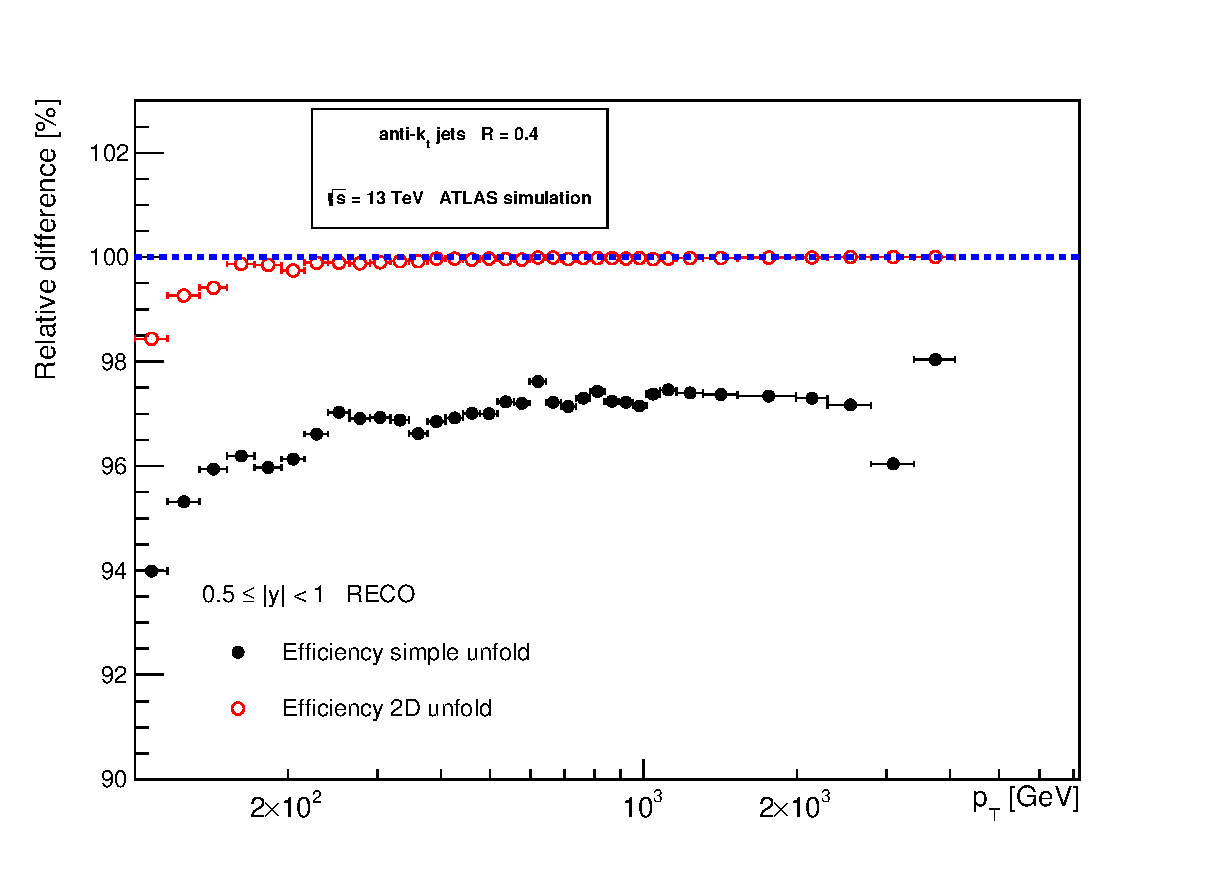
\includegraphics[width=0.49\textwidth]{{Chapter3/MatchEffSimpe2DSignal|abs(y)|0.5-1Compare}.eps}
  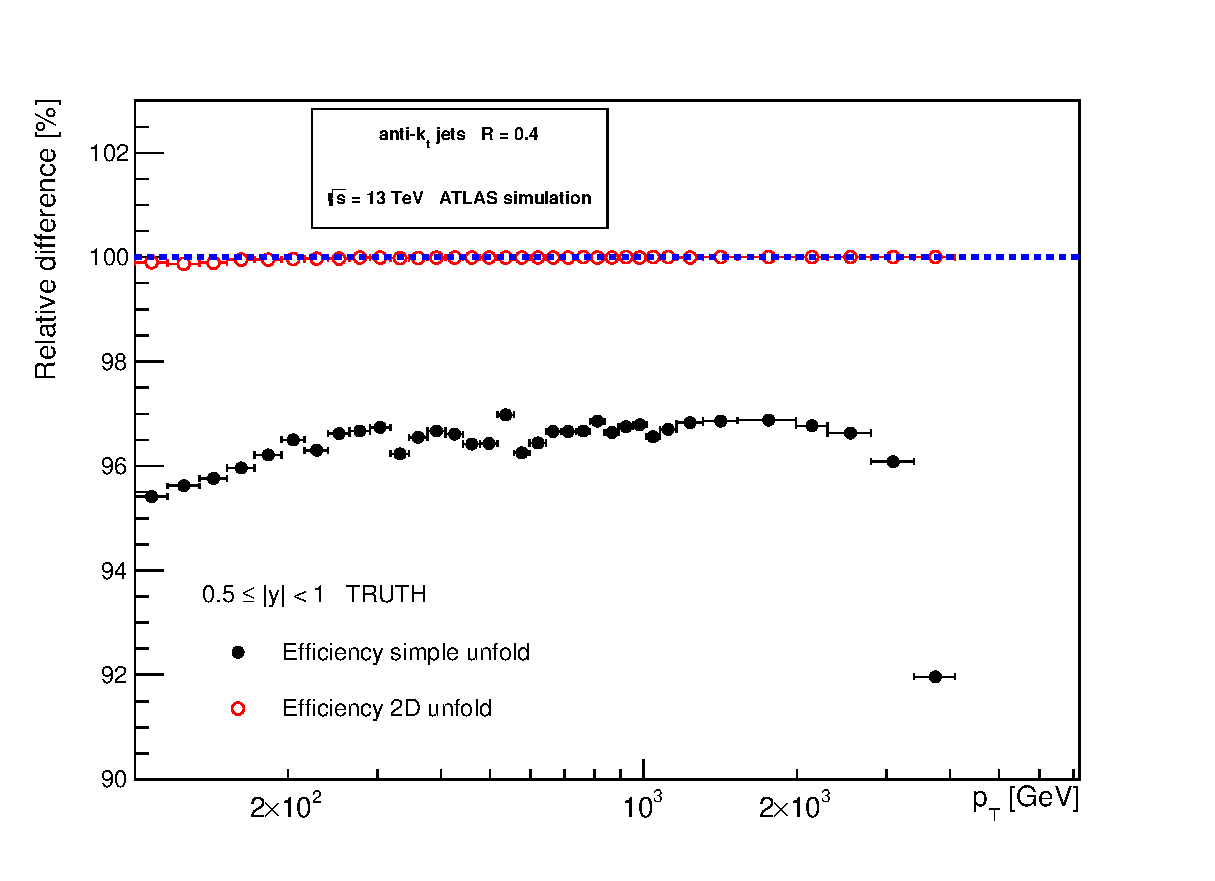
\includegraphics[width=0.49\textwidth]{{Chapter3/MatchEffSimpe2DTruth|abs(y)|0.5-1Compare}.eps}
  \caption{Comparison of matching efficiencies of simple and 2D unfolding for
  $|y| < 0.5$ (top) and $0.5 \leq |y| < 1$ (bottom) rapidity bins. Matching
  efficiencies are shown for both reco jets (left) and truth jets (right). }
\end{figure}

\begin{figure}[p]
  \centering
  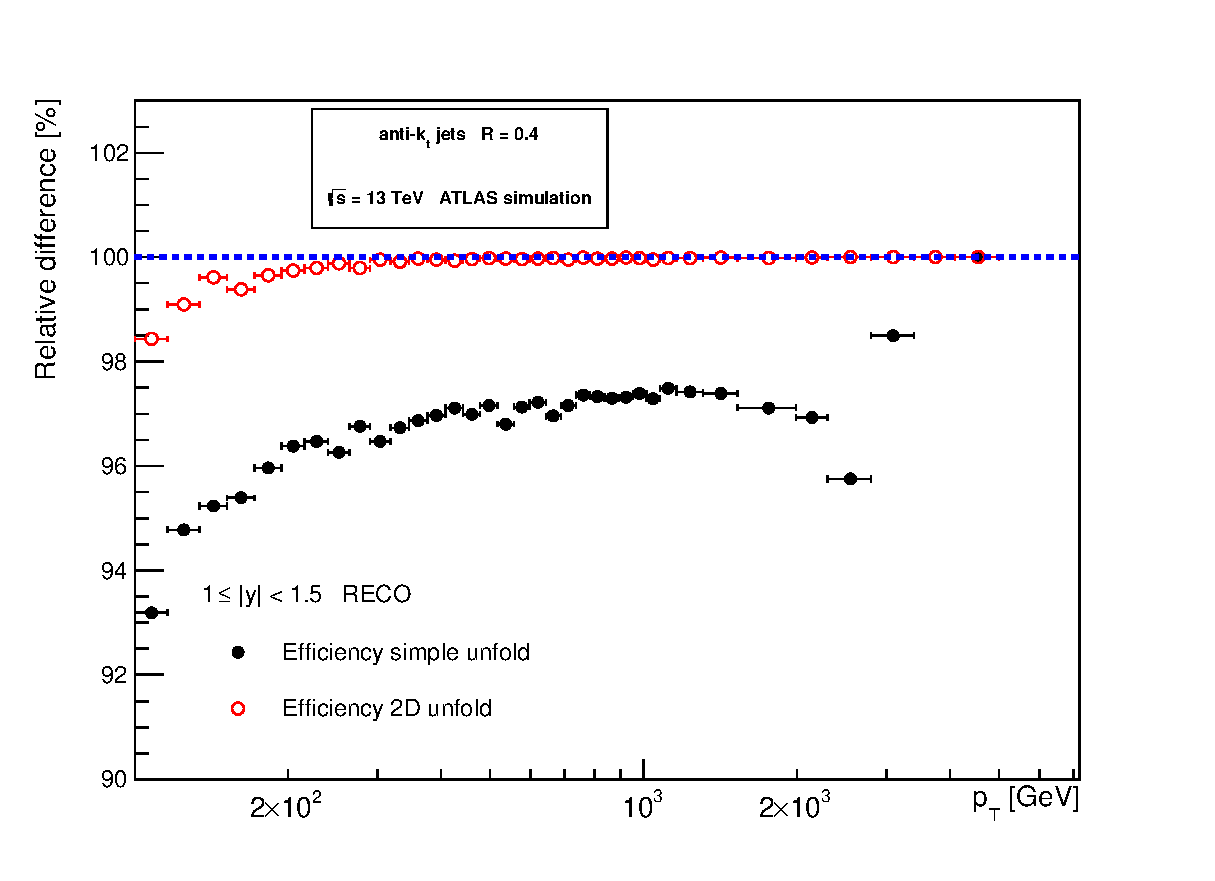
\includegraphics[width=0.49\textwidth]{{Chapter3/MatchEffSimpe2DSignal|abs(y)|1-1.5Compare}.eps}
  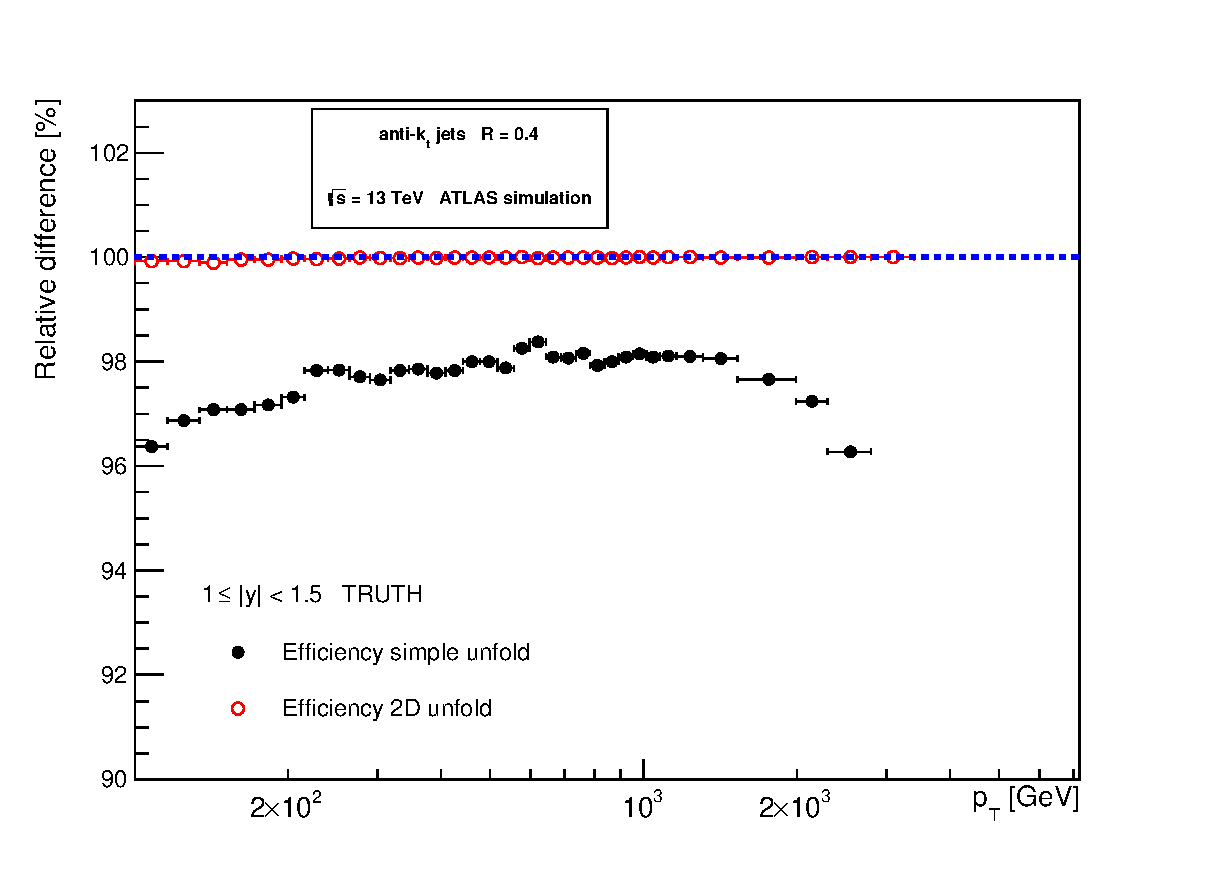
\includegraphics[width=0.49\textwidth]{{Chapter3/MatchEffSimpe2DTruth|abs(y)|1-1.5Compare}.eps}
  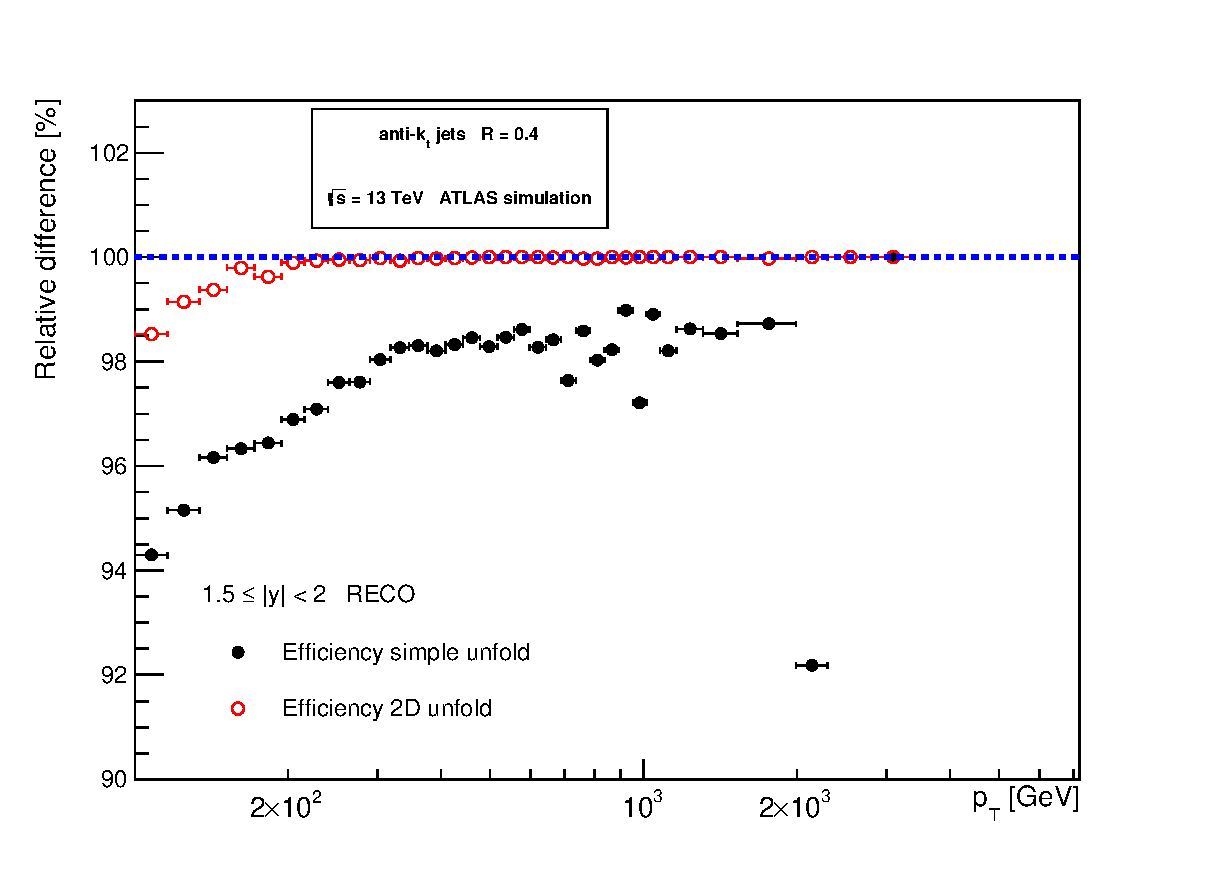
\includegraphics[width=0.49\textwidth]{{Chapter3/MatchEffSimpe2DSignal|abs(y)|1.5-2Compare}.eps}
  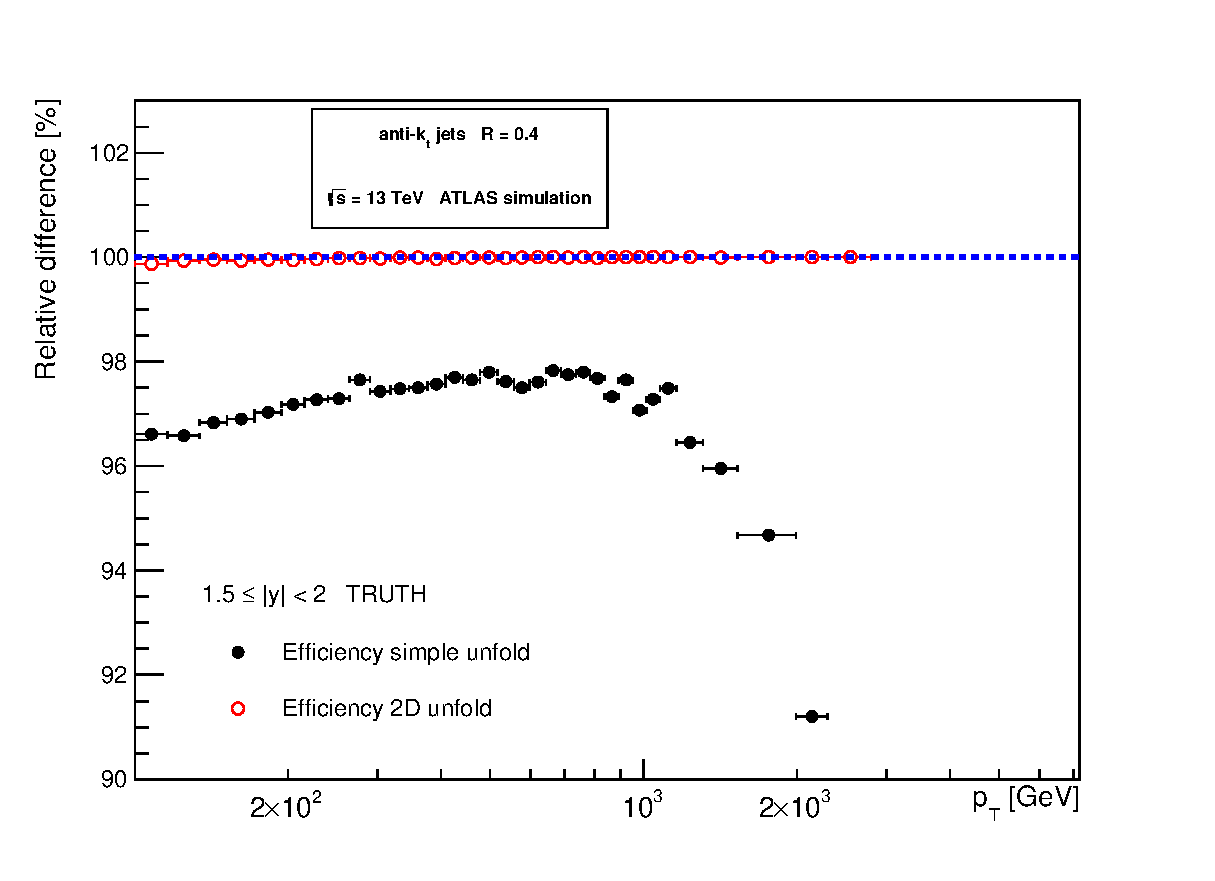
\includegraphics[width=0.49\textwidth]{{Chapter3/MatchEffSimpe2DTruth|abs(y)|1.5-2Compare}.eps}
  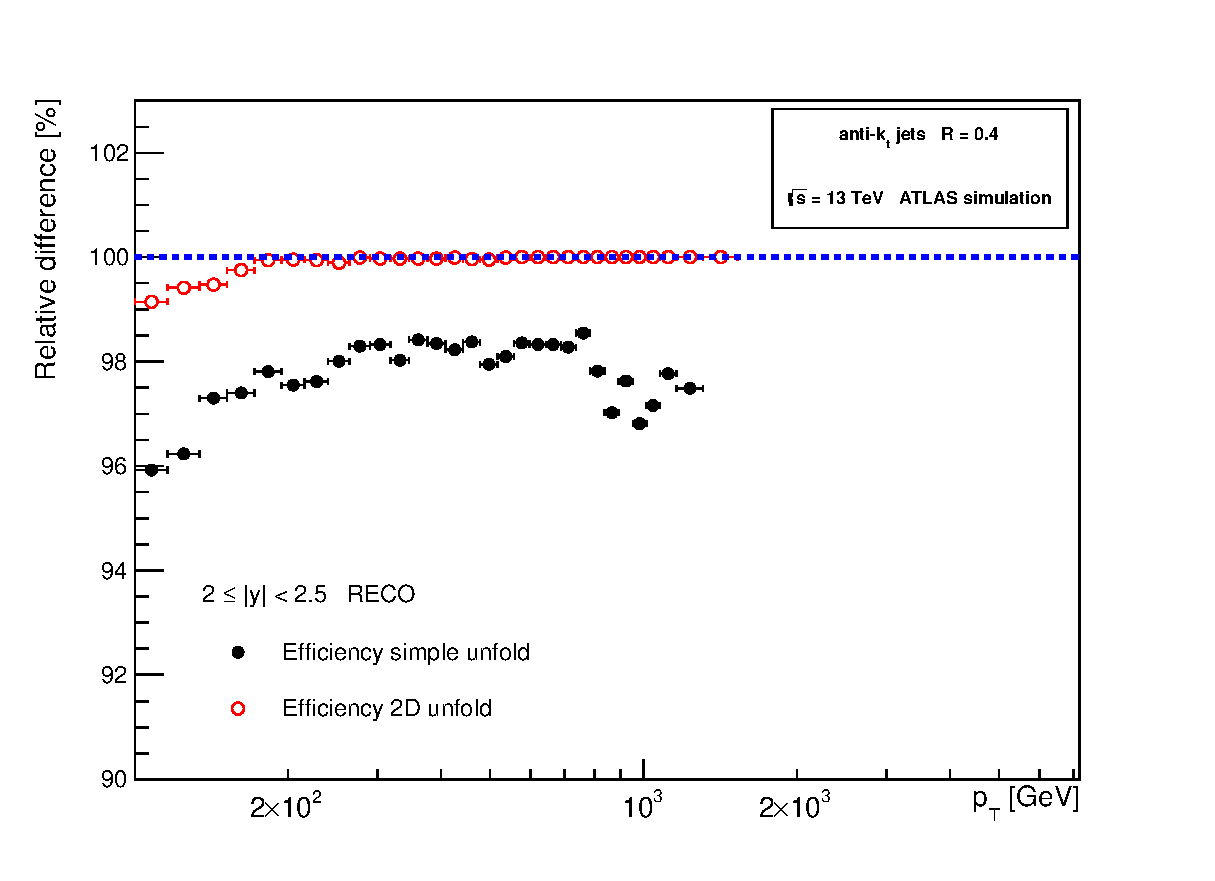
\includegraphics[width=0.49\textwidth]{{Chapter3/MatchEffSimpe2DSignal|abs(y)|2-2.5Compare}.eps}
  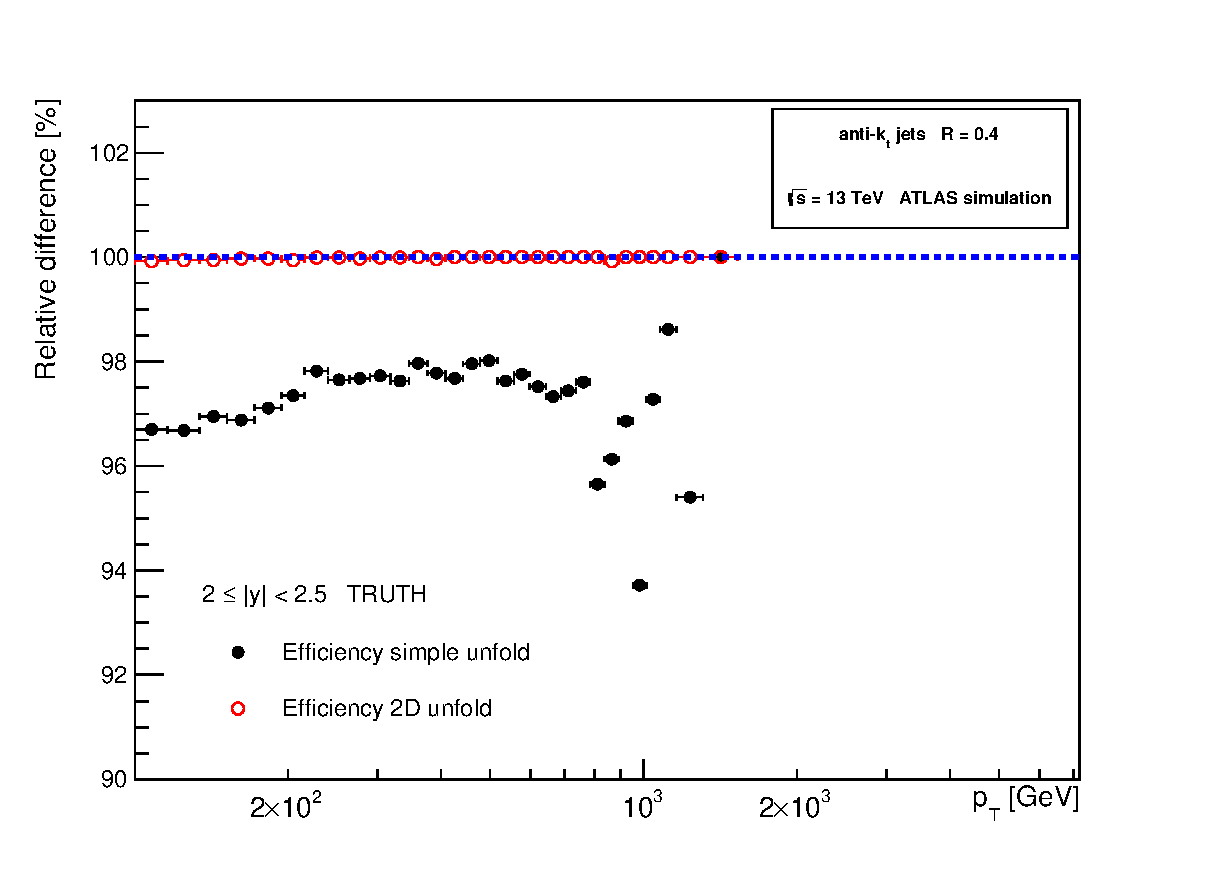
\includegraphics[width=0.49\textwidth]{{Chapter3/MatchEffSimpe2DTruth|abs(y)|2-2.5Compare}.eps}
  \caption{Comparison of matching efficiencies of simple and 2D unfolding for
  $1 \leq |y| < 1.5$ (top), $1.5 \leq |y| < 2$ and $2 \leq |y| < 2.5$ (bottom)
  rapidity bins. Matching efficiencies are shown for both reco jets (left) and truth
  jets (right). }
\end{figure}

\begin{figure}[p]
  \centering
  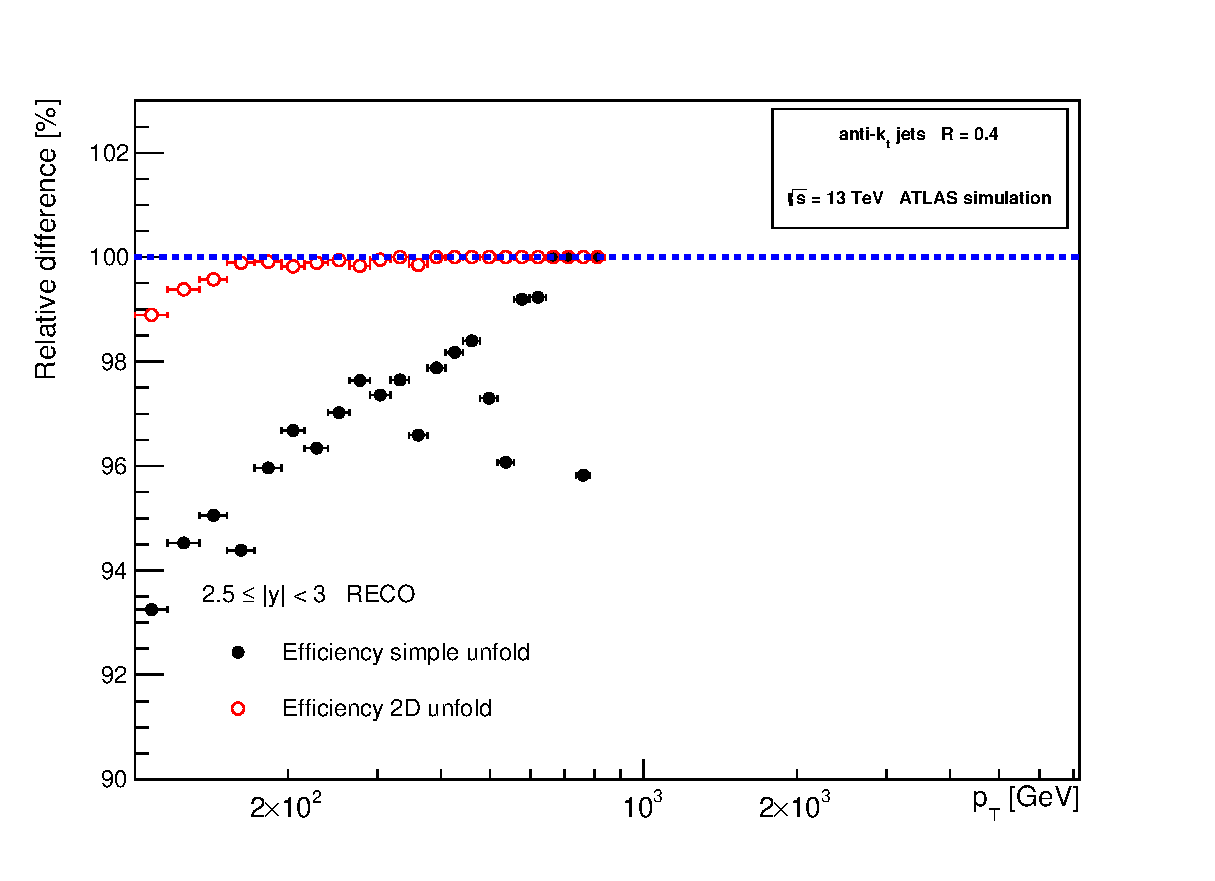
\includegraphics[width=0.49\textwidth]{{Chapter3/MatchEffSimpe2DSignal|abs(y)|2.5-3Compare}.eps}
  \includegraphics[width=0.49\textwidth]{{Chapter3/MatchEffSimpe2DTruth|abs(y)|2.5-3Compare}.eps}
  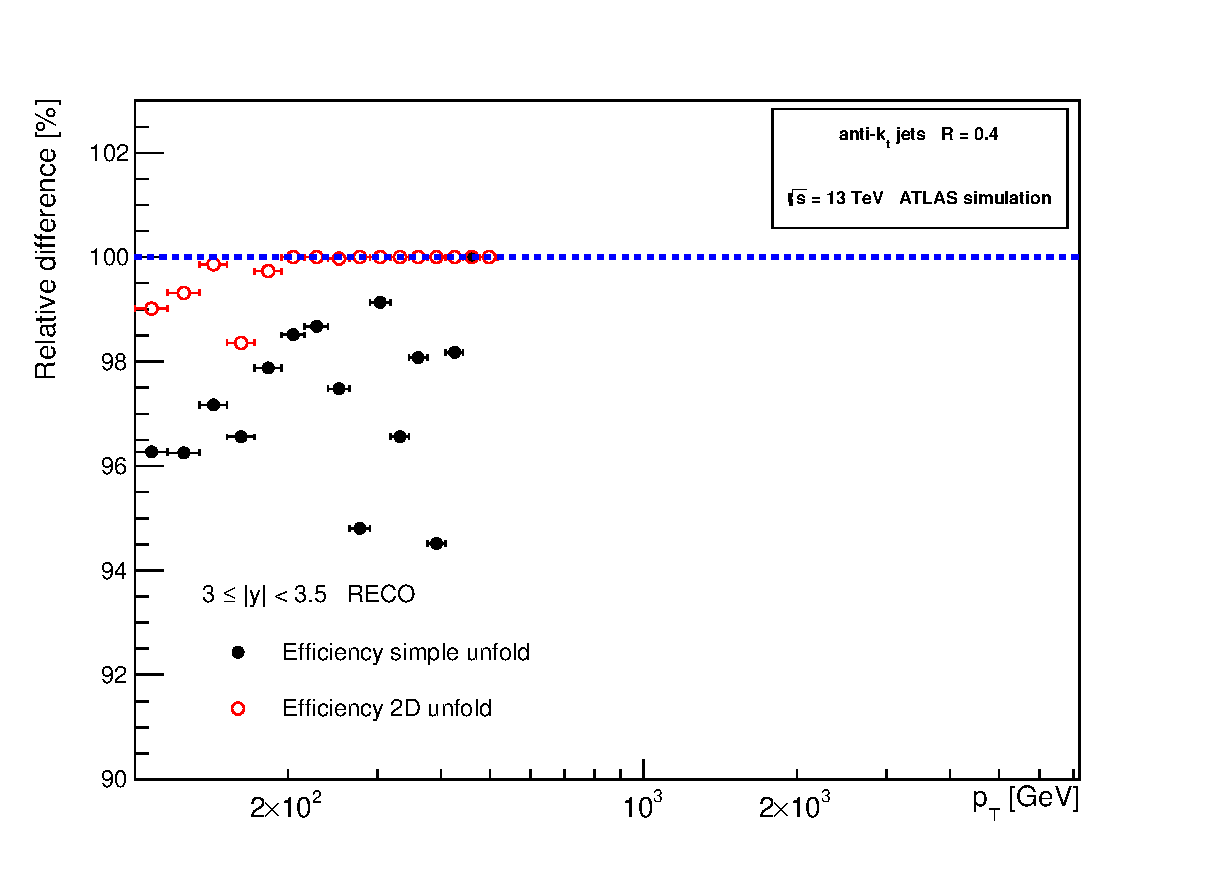
\includegraphics[width=0.49\textwidth]{{Chapter3/MatchEffSimpe2DSignal|abs(y)|3-3.5Compare}.eps}
  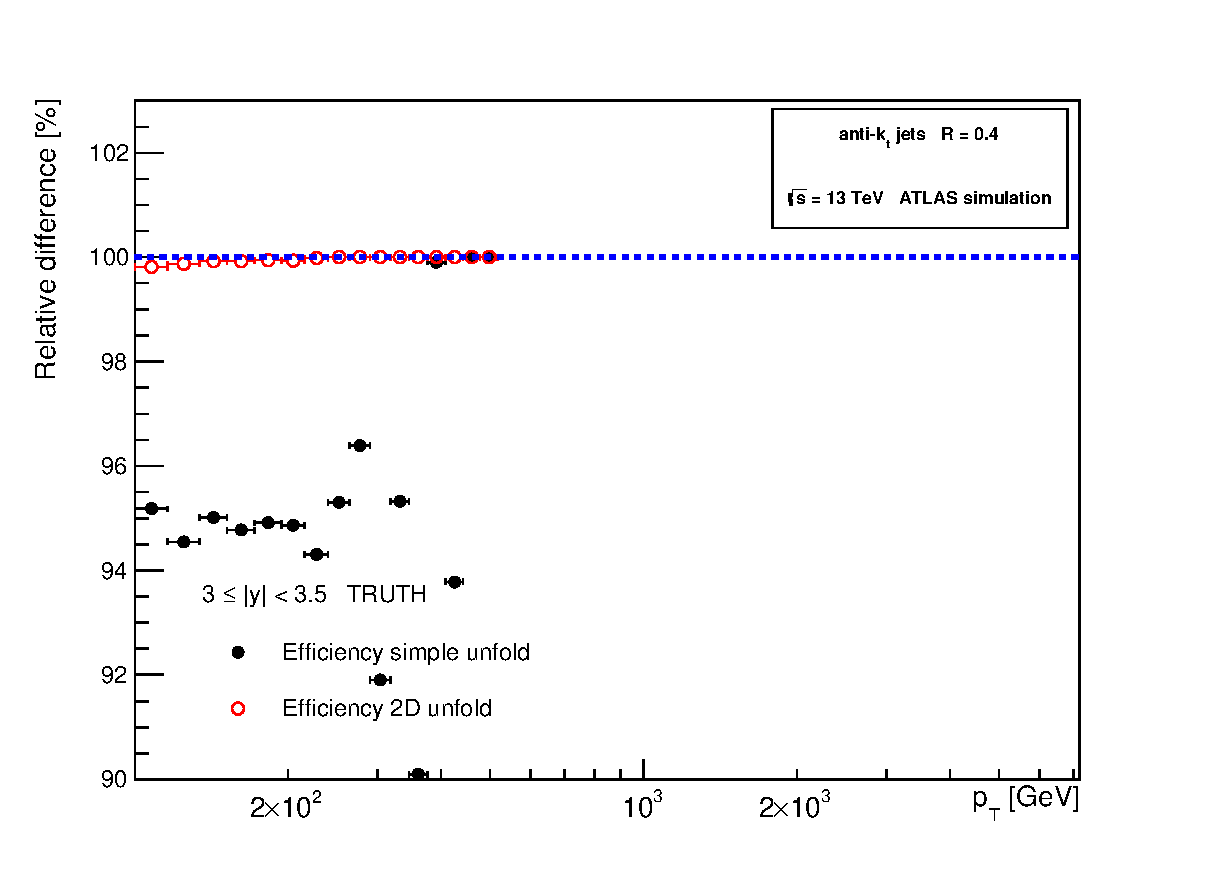
\includegraphics[width=0.49\textwidth]{{Chapter3/MatchEffSimpe2DTruth|abs(y)|3-3.5Compare}.eps}
  \includegraphics[width=0.49\textwidth]{{Chapter3/MatchEffSimpe2DSignal|abs(y)|3.5-4Compare}.eps}
  \includegraphics[width=0.49\textwidth]{{Chapter3/MatchEffSimpe2DTruth|abs(y)|3.5-4Compare}.eps}
  \caption{Comparison of matching efficiencies of simple and 2D unfolding for
  $2.5 \leq |y| < 3$ (top), $3 \leq |y| < 3.5$ and $3.5 \leq |y| < 4$ (bottom)
  rapidity bins. Matching efficiencies are shown for both reco jets (left) and truth
  jets (right). }
\end{figure}

\section{Unfolding Results}
\label{sec:UnfoldingResults}

\begin{figure}[H]
  \centering
  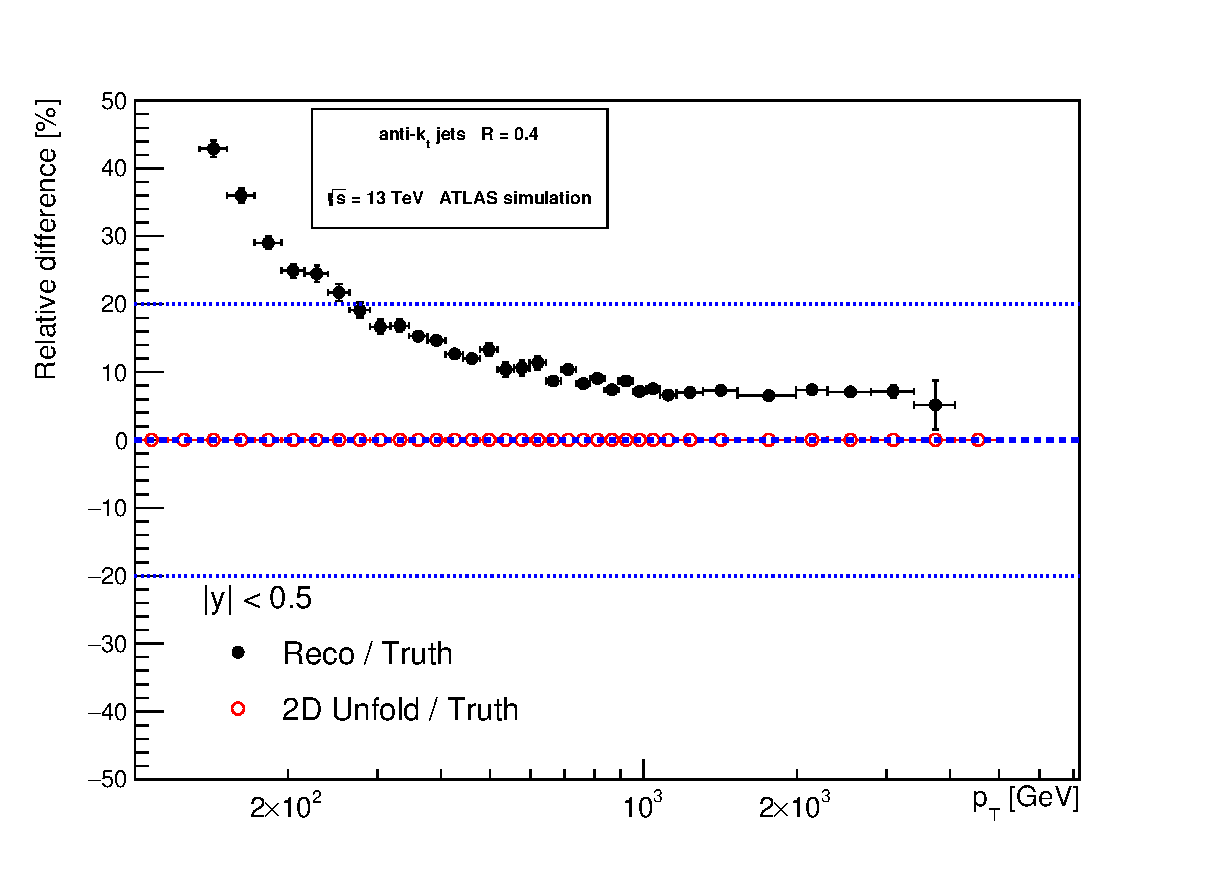
\includegraphics[width=0.49\textwidth]{{Chapter3/SignalUnfolded_VS_Truth|abs(y)|0-0.5Compare}.eps}
  \includegraphics[width=0.49\textwidth]{{Chapter3/SignalUnfolded_VS_Truth|abs(y)|0.5-1Compare}.eps}
  \includegraphics[width=0.49\textwidth]{{Chapter3/SignalUnfolded_VS_Truth|abs(y)|1-1.5Compare}.eps}
  \includegraphics[width=0.49\textwidth]{{Chapter3/SignalUnfolded_VS_Truth|abs(y)|1.5-2Compare}.eps}
  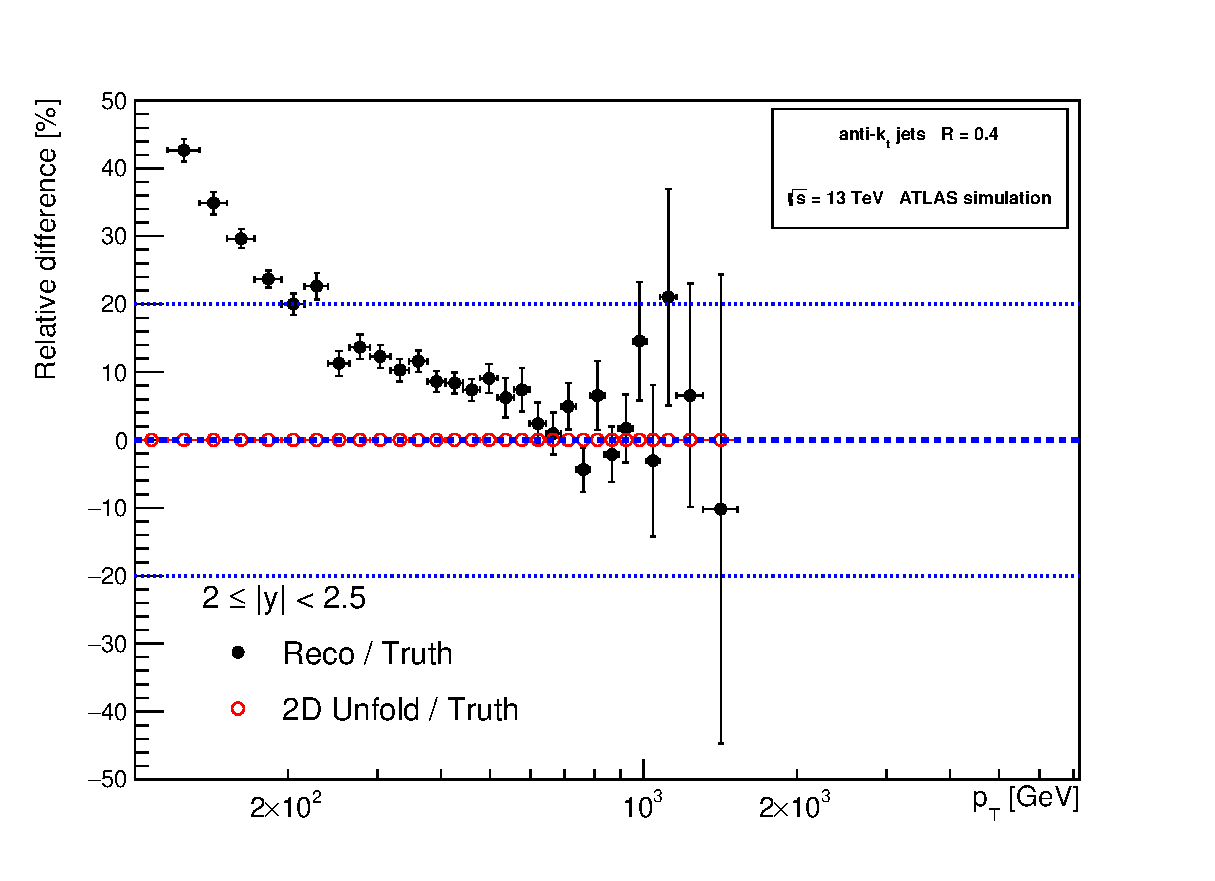
\includegraphics[width=0.49\textwidth]{{Chapter3/SignalUnfolded_VS_Truth|abs(y)|2-2.5Compare}.eps}
  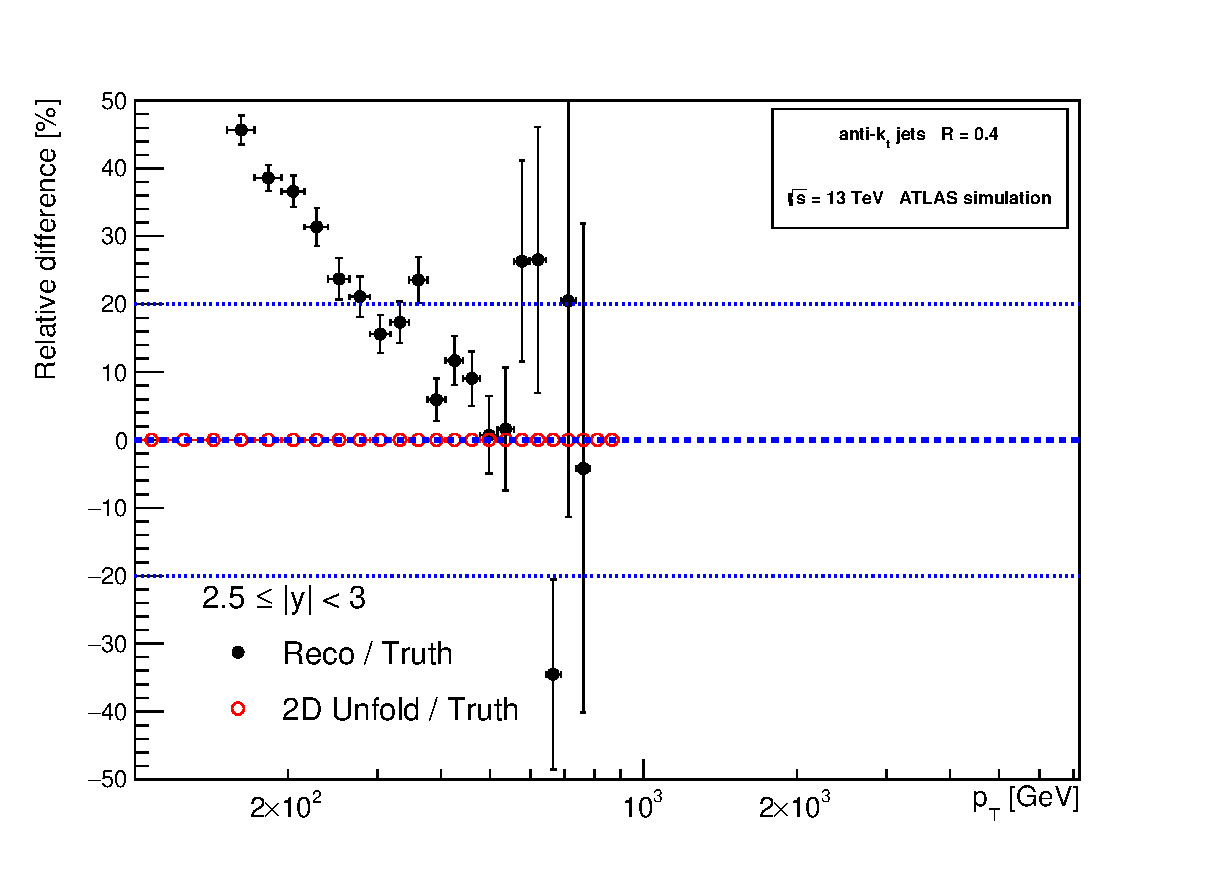
\includegraphics[width=0.49\textwidth]{{Chapter3/SignalUnfolded_VS_Truth|abs(y)|2.5-3Compare}.eps}
  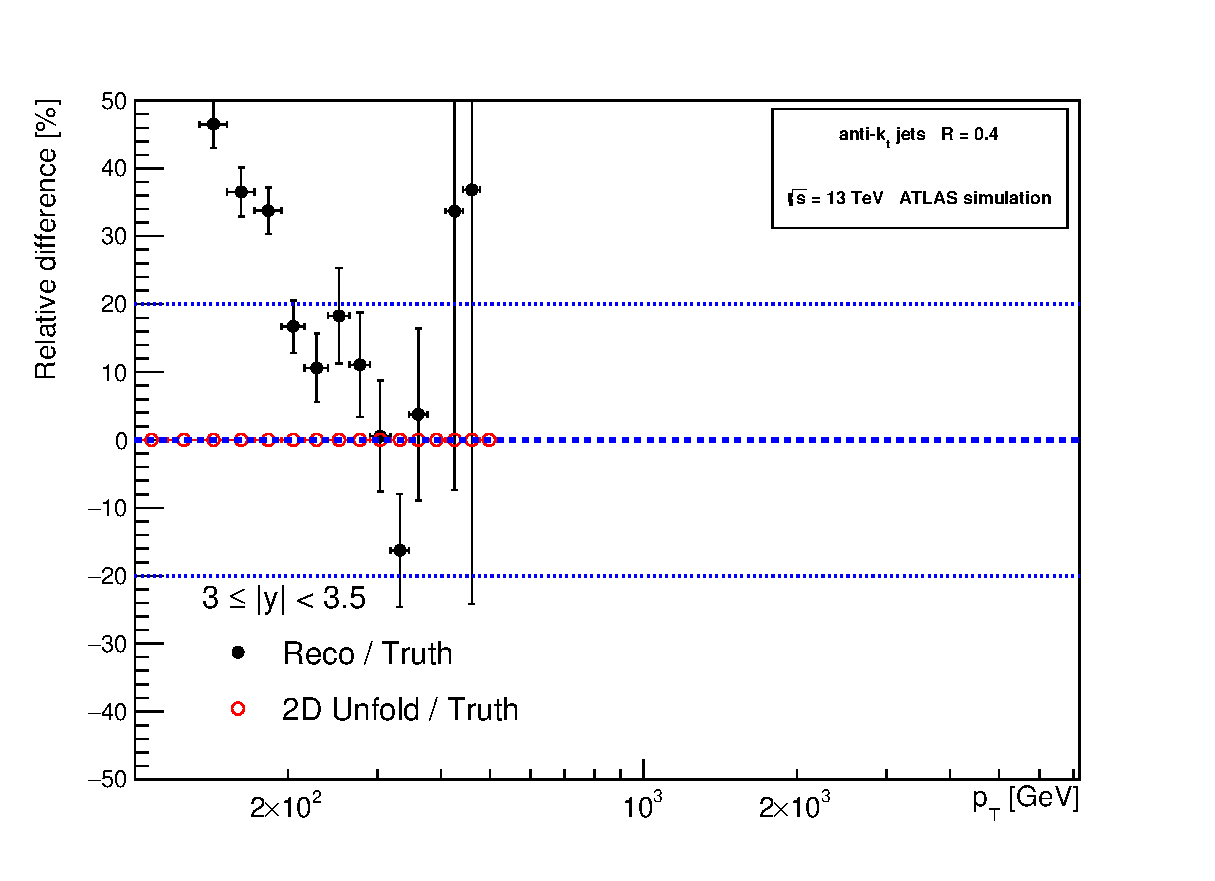
\includegraphics[width=0.49\textwidth]{{Chapter3/SignalUnfolded_VS_Truth|abs(y)|3-3.5Compare}.eps}
  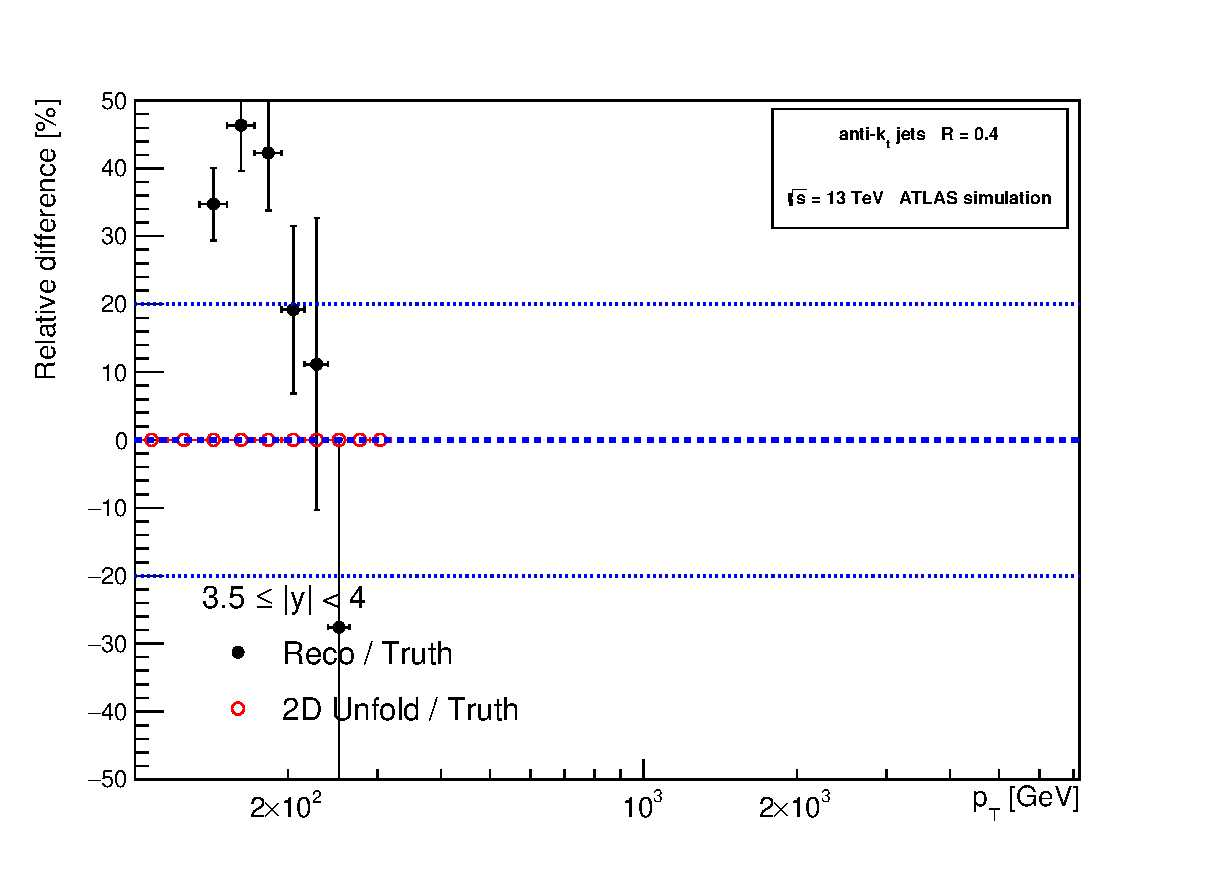
\includegraphics[width=0.49\textwidth]{{Chapter3/SignalUnfolded_VS_Truth|abs(y)|3.5-4Compare}.eps}
  \caption{Comparison of $\pt$ spectra of reco jets and the unfolded $\pt$
  spectra (2D unfolding) with the $\pt$ spectra of the truth jets for 8
  different rapidity bins.}
\end{figure}

\section{Simple and 2D Unfolding}
\label{sec:SimpleAnd2DUnfolding}

\begin{figure}[H]
  \centering
  \includegraphics[width=0.49\textwidth]{{Chapter3/UnfoldedSimpleComplex_VS_Truth|abs(y)|0-0.5Compare}.eps}
  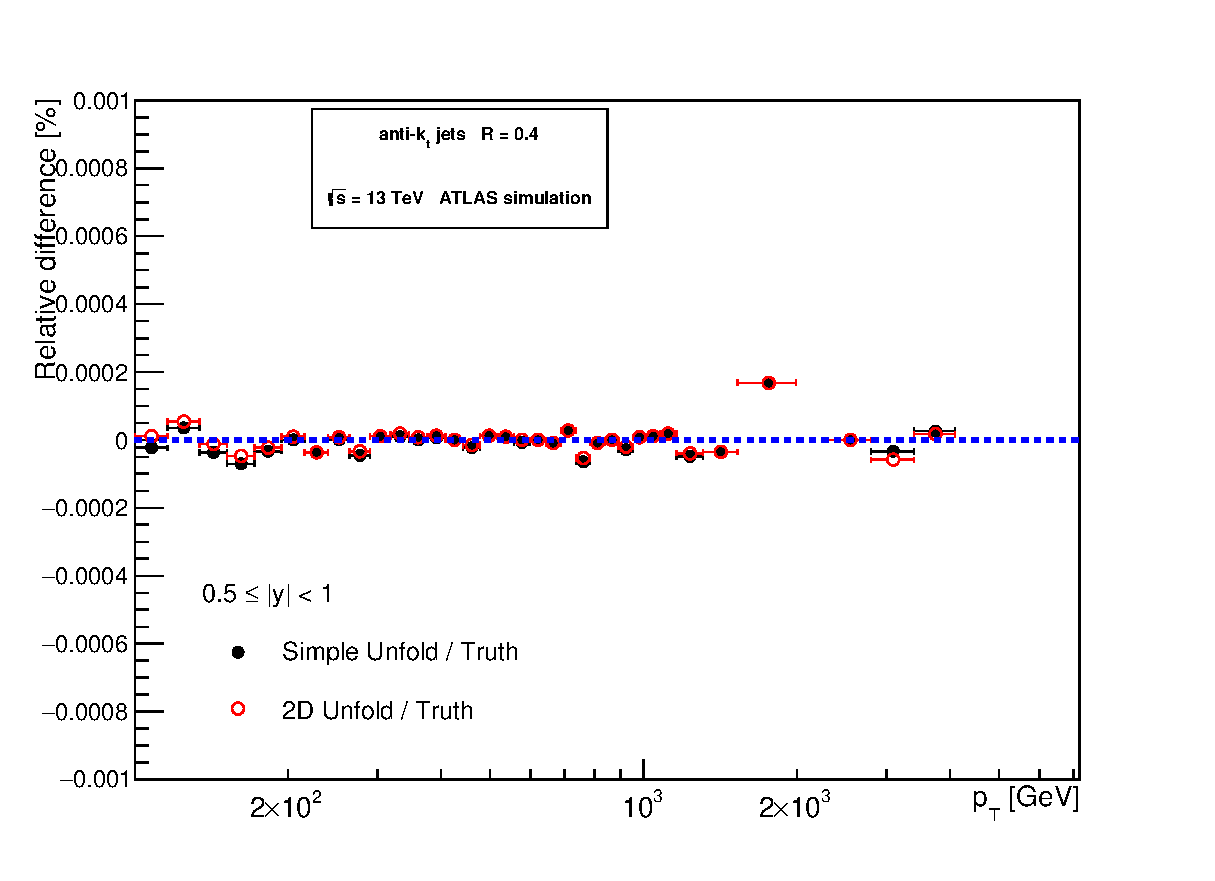
\includegraphics[width=0.49\textwidth]{{Chapter3/UnfoldedSimpleComplex_VS_Truth|abs(y)|0.5-1Compare}.eps}
  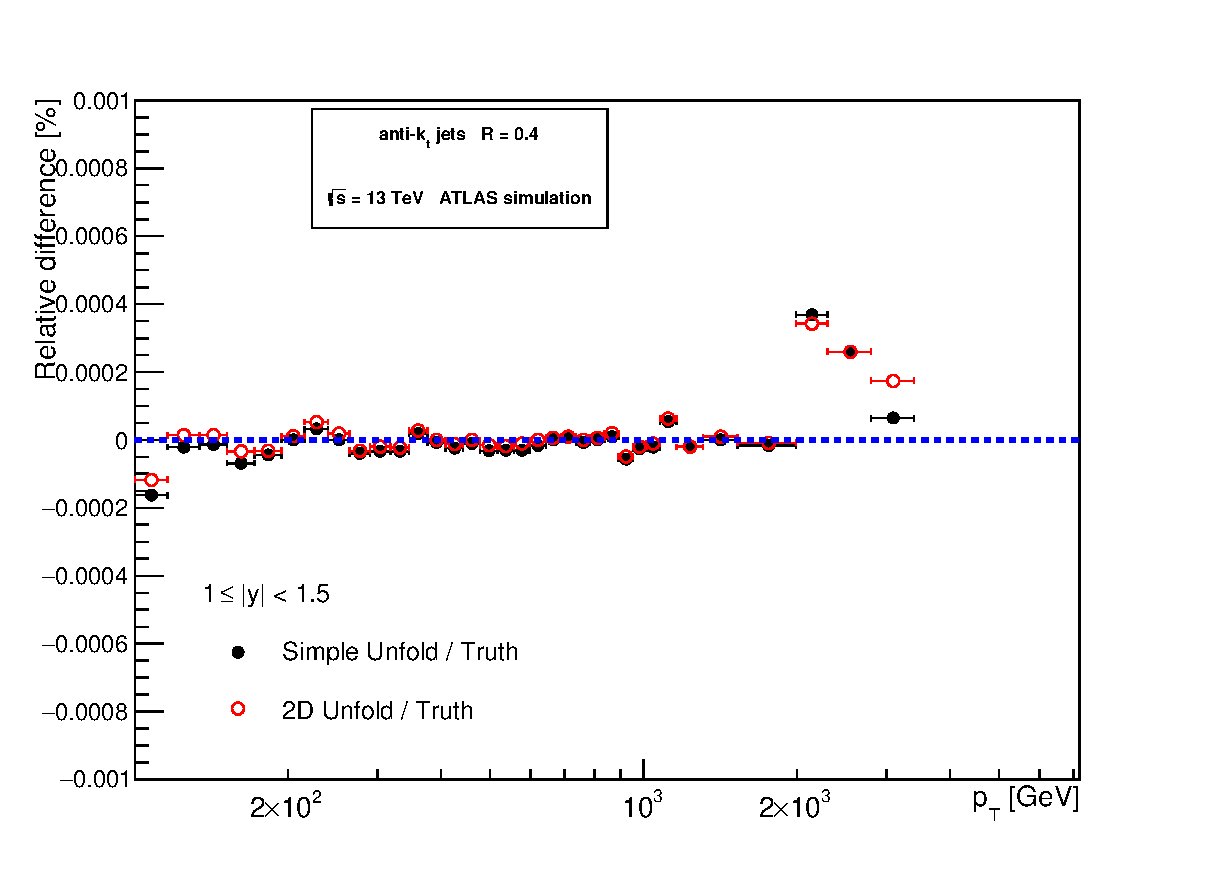
\includegraphics[width=0.49\textwidth]{{Chapter3/UnfoldedSimpleComplex_VS_Truth|abs(y)|1-1.5Compare}.eps}
  \includegraphics[width=0.49\textwidth]{{Chapter3/UnfoldedSimpleComplex_VS_Truth|abs(y)|1.5-2Compare}.eps}
  \includegraphics[width=0.49\textwidth]{{Chapter3/UnfoldedSimpleComplex_VS_Truth|abs(y)|2-2.5Compare}.eps}
  \includegraphics[width=0.49\textwidth]{{Chapter3/UnfoldedSimpleComplex_VS_Truth|abs(y)|2.5-3Compare}.eps}
  \includegraphics[width=0.49\textwidth]{{Chapter3/UnfoldedSimpleComplex_VS_Truth|abs(y)|3-3.5Compare}.eps}
  \includegraphics[width=0.49\textwidth]{{Chapter3/UnfoldedSimpleComplex_VS_Truth|abs(y)|3.5-4Compare}.eps}
  \caption{Comparison of results obtained by two unfolding method - simple and
    2D unfolding - with the $\pt$ spectra of truth jets for 8 different
    rapidity bins.}
\end{figure}

\chapter{NLO QCD Prediction}
\label{App:UnfoldingAndPrediction}

\newpage

\section{Predictions for Run I and Run II}
\label{sec:PredictionsForRunIAndII}

\begin{figure}[H]
  \centering
  \includegraphics[width=0.9\textwidth]{{Chapter3/PredictionCompare0}.eps}
  \includegraphics[width=0.9\textwidth]{{Chapter3/PredictionCompare1}.eps}
  \caption{Comparison of NLO QCD prediction of double differential inclusive jet
    cross section (black) in $\pt$ and rapidity of $pp$ collisions at $\rts=13\TeV$
    (filled circles) corresponding to LHC Run II and $\rts=8\TeV$ (empty circles)
    corresponding to LHC Run I. The cross section is multiplied by integrated
    luminosities and $\pt$ bin width to obtain expected number of jets observed in
    each $\pt$ bin (blue). Figures show the comparison for $0.5<|y|$ (top) and
    $0.5\leq|y|<1$ (bottom) rapidity bins.}
\end{figure}

\begin{figure}[p]
  \centering
  \includegraphics[width=0.9\textwidth]{{Chapter3/PredictionCompare2}.eps}
  \includegraphics[width=0.9\textwidth]{{Chapter3/PredictionCompare3}.eps}
  \caption{Comparison of NLO QCD prediction of double differential inclusive jet
    cross section (black) in $\pt$ and rapidity of $pp$ collisions at $\rts=13\TeV$
    (filled circles) corresponding to LHC Run II and $\rts=8\TeV$ (empty circles)
    corresponding to LHC Run I. The cross section is multiplied by integrated
    luminosities and $\pt$ bin width to obtain expected number of jets observed in
    each $\pt$ bin (blue). Figures show the comparison for $1\leq|y|<1.5$ (top) and $1.5
    \leq |y| < 2$ (bottom) rapidity bins.}
\end{figure}

\begin{figure}[p]
  \centering
  \includegraphics[width=0.9\textwidth]{{Chapter3/PredictionCompare4}.eps}
  \includegraphics[width=0.9\textwidth]{{Chapter3/PredictionCompare5}.eps}
  \caption{Comparison of NLO QCD prediction of double differential inclusive jet
    cross section (black) in $\pt$ and rapidity of $pp$ collisions at $\rts=13\TeV$
    (filled circles) corresponding to LHC Run II and $\rts=8\TeV$ (empty circles)
    corresponding to LHC Run I. The cross section is multiplied by integrated
    luminosities and $\pt$ bin width to obtain expected number of jets observed in
    each $\pt$ bin (blue). Figures show the comparison for $2\leq|y|<2.5$ (top) and $2.5
    \leq |y| < 3$ (bottom) rapidity bins.}
\end{figure}

\section{NLO Uncertainties}
\label{sec:NLOUncertainties}

\begin{figure}[H]
  \centering
  \includegraphics[width=0.49\textwidth]{{Chapter3/NLO_Systematics8_TeV0}.eps}
  \includegraphics[width=0.49\textwidth]{{Chapter3/NLO_Systematics13_TeV0}.eps}
  \includegraphics[width=0.49\textwidth]{{Chapter3/NLO_Systematics8_TeV1}.eps}
  \includegraphics[width=0.49\textwidth]{{Chapter3/NLO_Systematics13_TeV1}.eps}
  \includegraphics[width=0.49\textwidth]{{Chapter3/NLO_Systematics8_TeV2}.eps}
  \includegraphics[width=0.49\textwidth]{{Chapter3/NLO_Systematics13_TeV2}.eps}
  \caption{NLO uncertainties for NLO QCD predictions of inclusive jet double
    differential cross section of $pp$ collisions at $\rts=8\TeV$ (left) and
    $\rts=13\TeV$ (right) for $|y|<0.5$ (top), $0.5\leq|y|<1$ (middle) and
    $1\leq|y|<1.5$ (bottom) rapidity bins.}
\end{figure}

\begin{figure}[p]
  \centering
  \includegraphics[width=0.49\textwidth]{{Chapter3/NLO_Systematics8_TeV3}.eps}
  \includegraphics[width=0.49\textwidth]{{Chapter3/NLO_Systematics13_TeV3}.eps}
  \includegraphics[width=0.49\textwidth]{{Chapter3/NLO_Systematics8_TeV4}.eps}
  \includegraphics[width=0.49\textwidth]{{Chapter3/NLO_Systematics13_TeV4}.eps}
  \includegraphics[width=0.49\textwidth]{{Chapter3/NLO_Systematics8_TeV5}.eps}
  \includegraphics[width=0.49\textwidth]{{Chapter3/NLO_Systematics13_TeV5}.eps}
  \caption{NLO uncertainties for NLO QCD predictions of inclusive jet double
    differential cross section of $pp$ collisions at $\rts=8\TeV$ (left) and
    $\rts=13\TeV$ (right) for $1.5\leq|y|<2$ (top), $2\leq|y|<2.5$ (middle) and
    $2.5\leq|y|<3$ (bottom) rapidity bins.}
\end{figure}

\section{Pythia and NLO}
\label{sec:PythiaAndNLO}

\begin{figure}[H]
  \centering
  \includegraphics[width=0.49\textwidth]{{Chapter3/Truth_VS_Prediction|abs(y)|0-0.5Compare}.eps}
  \includegraphics[width=0.49\textwidth]{{Chapter3/Truth_VS_Prediction|abs(y)|0.5-1Compare}.eps}
  \includegraphics[width=0.49\textwidth]{{Chapter3/Truth_VS_Prediction|abs(y)|1-1.5Compare}.eps}
  \includegraphics[width=0.49\textwidth]{{Chapter3/Truth_VS_Prediction|abs(y)|1.5-2Compare}.eps}
  \includegraphics[width=0.49\textwidth]{{Chapter3/Truth_VS_Prediction|abs(y)|2-2.5Compare}.eps}
  \includegraphics[width=0.49\textwidth]{{Chapter3/Truth_VS_Prediction|abs(y)|2.5-3Compare}.eps}
  \caption{Comparison of \textsc{Pythia8} prediction with NLO QCD prediction of
    inclusive jet double differential cross section in $\pt$ and rapidity for six
    different rapidity bins. Blue area represents the uncertainties of NLO QCD
    predictions.}
\end{figure}

\end{appendices}



%================================================================================
% Bibliografie
%================================================================================

\clearpage
\addcontentsline{toc}{chapter}{Bibliography}
\bibliographystyle{ieeetr}
\bibliography{bibliography}

\cleardoublepage

%\clearpage
%
%\MyQuote{Physics is the only profession in which prophecy is not only accurate but
%routine.}{Neil deGrasse Tyson}
%
%\MyQuote{If you wish to understand the Universe, think of energy, frequency and
%vibration.}{Nikola Tesla}
%
%\MyQuote{In physics, you don't have to go around making trouble for yourself - nature
%does it for you.}{Frank Wilczek}
%
%\MyQuote{Every wave, regardless of how high and forceful it crests, must eventually
%collapse within itself.}{Stefan Zweig}
%
%\MyQuote{There is no certainty in sciences where one of the mathematical sciences cannot
%be applied, or which are not in relation with these mathematics.}{Leonardo da Vinci}
%
%\MyQuote{I think that modern physics has definitely decided in favor of Plato. In fact
%the smallest units of matter are not physical objects in the ordinary sense;
%they are forms, ideas which can be expressed unambiguously only in mathematical
%language.}{Werner Heisenberg}
%
%\MyQuote{To confine our attention to terrestrial matters would be to limit the
%human spirit.}{Stephen Hawking}

\end{document}
